\documentclass[twoside]{book}

% Packages required by doxygen
\usepackage{fixltx2e}
\usepackage{calc}
\usepackage{doxygen}
\usepackage[export]{adjustbox} % also loads graphicx
\usepackage{graphicx}
\usepackage[utf8]{inputenc}
\usepackage{makeidx}
\usepackage{multicol}
\usepackage{multirow}
\PassOptionsToPackage{warn}{textcomp}
\usepackage{textcomp}
\usepackage[nointegrals]{wasysym}
\usepackage[table]{xcolor}

% Font selection
\usepackage[T1]{fontenc}
\usepackage[scaled=.90]{helvet}
\usepackage{courier}
\usepackage{amssymb}
\usepackage{sectsty}
\renewcommand{\familydefault}{\sfdefault}
\allsectionsfont{%
  \fontseries{bc}\selectfont%
  \color{darkgray}%
}
\renewcommand{\DoxyLabelFont}{%
  \fontseries{bc}\selectfont%
  \color{darkgray}%
}
\newcommand{\+}{\discretionary{\mbox{\scriptsize$\hookleftarrow$}}{}{}}

% Page & text layout
\usepackage{geometry}
\geometry{%
  a4paper,%
  top=2.5cm,%
  bottom=2.5cm,%
  left=2.5cm,%
  right=2.5cm%
}
\tolerance=750
\hfuzz=15pt
\hbadness=750
\setlength{\emergencystretch}{15pt}
\setlength{\parindent}{0cm}
\setlength{\parskip}{3ex plus 2ex minus 2ex}
\makeatletter
\renewcommand{\paragraph}{%
  \@startsection{paragraph}{4}{0ex}{-1.0ex}{1.0ex}{%
    \normalfont\normalsize\bfseries\SS@parafont%
  }%
}
\renewcommand{\subparagraph}{%
  \@startsection{subparagraph}{5}{0ex}{-1.0ex}{1.0ex}{%
    \normalfont\normalsize\bfseries\SS@subparafont%
  }%
}
\makeatother

% Headers & footers
\usepackage{fancyhdr}
\pagestyle{fancyplain}
\fancyhead[LE]{\fancyplain{}{\bfseries\thepage}}
\fancyhead[CE]{\fancyplain{}{}}
\fancyhead[RE]{\fancyplain{}{\bfseries\leftmark}}
\fancyhead[LO]{\fancyplain{}{\bfseries\rightmark}}
\fancyhead[CO]{\fancyplain{}{}}
\fancyhead[RO]{\fancyplain{}{\bfseries\thepage}}
\fancyfoot[LE]{\fancyplain{}{}}
\fancyfoot[CE]{\fancyplain{}{}}
\fancyfoot[RE]{\fancyplain{}{\bfseries\scriptsize 制作者 Doxygen }}
\fancyfoot[LO]{\fancyplain{}{\bfseries\scriptsize 制作者 Doxygen }}
\fancyfoot[CO]{\fancyplain{}{}}
\fancyfoot[RO]{\fancyplain{}{}}
\renewcommand{\footrulewidth}{0.4pt}
\renewcommand{\chaptermark}[1]{%
  \markboth{#1}{}%
}
\renewcommand{\sectionmark}[1]{%
  \markright{\thesection\ #1}%
}

% Indices & bibliography
\usepackage{natbib}
\usepackage[titles]{tocloft}
\setcounter{tocdepth}{3}
\setcounter{secnumdepth}{5}
\makeindex

% Hyperlinks (required, but should be loaded last)
\usepackage{ifpdf}
\ifpdf
  \usepackage[pdftex,pagebackref=true]{hyperref}
\else
  \usepackage[ps2pdf,pagebackref=true]{hyperref}
\fi
\hypersetup{%
  colorlinks=true,%
  linkcolor=blue,%
  citecolor=blue,%
  unicode%
}

% Custom commands
\newcommand{\clearemptydoublepage}{%
  \newpage{\pagestyle{empty}\cleardoublepage}%
}

\usepackage{caption}
\captionsetup{labelsep=space,justification=centering,font={bf},singlelinecheck=off,skip=4pt,position=top}

%===== C O N T E N T S =====

\begin{document}

% Titlepage & ToC
\hypersetup{pageanchor=false,
             bookmarksnumbered=true,
             pdfencoding=unicode
            }
\pagenumbering{alph}
\begin{titlepage}
\vspace*{7cm}
\begin{center}%
{\Large 数据结构课设 \\[1ex]\large beta 1.\+0 }\\
\vspace*{1cm}
{\large 制作者 Doxygen 1.8.13}\\
\end{center}
\end{titlepage}
\clearemptydoublepage
\pagenumbering{roman}
\tableofcontents
\clearemptydoublepage
\pagenumbering{arabic}
\hypersetup{pageanchor=true}

%--- Begin generated contents ---
\chapter{类索引}
\section{类列表}
这里列出了所有类、结构、联合以及接口定义等,并附带简要说明\+:\begin{DoxyCompactList}
\item\contentsline{section}{\hyperlink{struct_b_i_n_t_r_e_e}{B\+I\+N\+T\+R\+EE} }{\pageref{struct_b_i_n_t_r_e_e}}{}
\item\contentsline{section}{\hyperlink{struct_m_e_m_b_e_r_n_o_d_e}{M\+E\+M\+B\+E\+R\+N\+O\+DE} }{\pageref{struct_m_e_m_b_e_r_n_o_d_e}}{}
\item\contentsline{section}{\hyperlink{struct_r_e_s_n_o_d_e}{R\+E\+S\+N\+O\+DE} }{\pageref{struct_r_e_s_n_o_d_e}}{}
\item\contentsline{section}{\hyperlink{struct_s_t_a_c_k_n_o_d_e}{S\+T\+A\+C\+K\+N\+O\+DE} }{\pageref{struct_s_t_a_c_k_n_o_d_e}}{}
\end{DoxyCompactList}

\chapter{文件索引}
\section{文件列表}
这里列出了所有文件,并附带简要说明\+:\begin{DoxyCompactList}
\item\contentsline{section}{\hyperlink{_b_i_n_node_8h}{B\+I\+N\+Node.\+h} }{\pageref{_b_i_n_node_8h}}{}
\item\contentsline{section}{\hyperlink{_clear_hash_8h}{Clear\+Hash.\+h} }{\pageref{_clear_hash_8h}}{}
\item\contentsline{section}{\hyperlink{_clear_res_list_8h}{Clear\+Res\+List.\+h} }{\pageref{_clear_res_list_8h}}{}
\item\contentsline{section}{\hyperlink{_cont_exec_8h}{Cont\+Exec.\+h} }{\pageref{_cont_exec_8h}}{}
\item\contentsline{section}{\hyperlink{_d_l_r_search_bin_tree_8h}{D\+L\+R\+Search\+Bin\+Tree.\+h} }{\pageref{_d_l_r_search_bin_tree_8h}}{}
\item\contentsline{section}{\hyperlink{_file_read_8h}{File\+Read.\+h} }{\pageref{_file_read_8h}}{}
\item\contentsline{section}{\hyperlink{_file_write_8h}{File\+Write.\+h} }{\pageref{_file_write_8h}}{}
\item\contentsline{section}{\hyperlink{_function_8h}{Function.\+h} }{\pageref{_function_8h}}{}
\item\contentsline{section}{\hyperlink{_hash_cmp_8h}{Hash\+Cmp.\+h} }{\pageref{_hash_cmp_8h}}{}
\item\contentsline{section}{\hyperlink{_init_g_u_i_8h}{Init\+G\+U\+I.\+h} }{\pageref{_init_g_u_i_8h}}{}
\item\contentsline{section}{\hyperlink{ins_bin_tree_8h}{ins\+Bin\+Tree.\+h} }{\pageref{ins_bin_tree_8h}}{}
\item\contentsline{section}{\hyperlink{ins_hash_8h}{ins\+Hash.\+h} }{\pageref{ins_hash_8h}}{}
\item\contentsline{section}{\hyperlink{_ins_res_list_8h}{Ins\+Res\+List.\+h} }{\pageref{_ins_res_list_8h}}{}
\item\contentsline{section}{\hyperlink{is_chinese_8h}{is\+Chinese.\+h} }{\pageref{is_chinese_8h}}{}
\item\contentsline{section}{\hyperlink{is_empty_stack_8h}{is\+Empty\+Stack.\+h} }{\pageref{is_empty_stack_8h}}{}
\item\contentsline{section}{\hyperlink{_k_m_p_8h}{K\+M\+P.\+h} }{\pageref{_k_m_p_8h}}{}
\item\contentsline{section}{\hyperlink{_l_r_d_clear_bin_tree_8h}{L\+R\+D\+Clear\+Bin\+Tree.\+h} }{\pageref{_l_r_d_clear_bin_tree_8h}}{}
\item\contentsline{section}{\hyperlink{_l_r_d_visit_bin_tree_8h}{L\+R\+D\+Visit\+Bin\+Tree.\+h} }{\pageref{_l_r_d_visit_bin_tree_8h}}{}
\item\contentsline{section}{\hyperlink{_member_node_8h}{Member\+Node.\+h} }{\pageref{_member_node_8h}}{}
\item\contentsline{section}{\hyperlink{_pop_stack_8h}{Pop\+Stack.\+h} }{\pageref{_pop_stack_8h}}{}
\item\contentsline{section}{\hyperlink{_push_stack_8h}{Push\+Stack.\+h} }{\pageref{_push_stack_8h}}{}
\item\contentsline{section}{\hyperlink{_quick_sort_8h}{Quick\+Sort.\+h} }{\pageref{_quick_sort_8h}}{}
\item\contentsline{section}{\hyperlink{res_node_8h}{res\+Node.\+h} }{\pageref{res_node_8h}}{}
\item\contentsline{section}{\hyperlink{rms_8c}{rms.\+c} }{\pageref{rms_8c}}{}
\item\contentsline{section}{\hyperlink{_search_hash_8h}{Search\+Hash.\+h} }{\pageref{_search_hash_8h}}{}
\item\contentsline{section}{\hyperlink{_show_result_8h}{Show\+Result.\+h} }{\pageref{_show_result_8h}}{}
\item\contentsline{section}{\hyperlink{_s_t_a_c_k_n_o_d_e_8h}{S\+T\+A\+C\+K\+N\+O\+D\+E.\+h} }{\pageref{_s_t_a_c_k_n_o_d_e_8h}}{}
\end{DoxyCompactList}

\chapter{类说明}
\hypertarget{struct_b_i_n_t_r_e_e}{}\section{B\+I\+N\+T\+R\+E\+E结构体 参考}
\label{struct_b_i_n_t_r_e_e}\index{B\+I\+N\+T\+R\+EE@{B\+I\+N\+T\+R\+EE}}


{\ttfamily \#include $<$B\+I\+N\+Node.\+h$>$}



B\+I\+N\+T\+R\+EE 的协作图\+:
\nopagebreak
\begin{figure}[H]
\begin{center}
\leavevmode
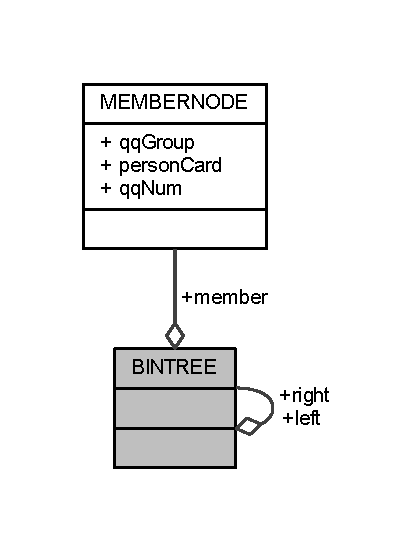
\includegraphics[width=199pt]{struct_b_i_n_t_r_e_e__coll__graph}
\end{center}
\end{figure}
\subsection*{Public 属性}
\begin{DoxyCompactItemize}
\item 
struct \hyperlink{struct_m_e_m_b_e_r_n_o_d_e}{M\+E\+M\+B\+E\+R\+N\+O\+DE} $\ast$ \hyperlink{struct_b_i_n_t_r_e_e_a3ab2c8b4cbbacb80e686e334208c5d48}{member}
\item 
struct \hyperlink{struct_b_i_n_t_r_e_e}{B\+I\+N\+T\+R\+EE} $\ast$ \hyperlink{struct_b_i_n_t_r_e_e_a4186a51481617735e0ad0ddc859a7ebf}{left}
\item 
struct \hyperlink{struct_b_i_n_t_r_e_e}{B\+I\+N\+T\+R\+EE} $\ast$ \hyperlink{struct_b_i_n_t_r_e_e_abe35ee9da1117f8df6d969647ad5ee19}{right}
\end{DoxyCompactItemize}


\subsection{详细描述}


在文件 B\+I\+N\+Node.\+h 第 4 行定义.



\subsection{类成员变量说明}
\mbox{\Hypertarget{struct_b_i_n_t_r_e_e_a4186a51481617735e0ad0ddc859a7ebf}\label{struct_b_i_n_t_r_e_e_a4186a51481617735e0ad0ddc859a7ebf}} 
\index{B\+I\+N\+T\+R\+EE@{B\+I\+N\+T\+R\+EE}!left@{left}}
\index{left@{left}!B\+I\+N\+T\+R\+EE@{B\+I\+N\+T\+R\+EE}}
\subsubsection{\texorpdfstring{left}{left}}
{\footnotesize\ttfamily struct \hyperlink{struct_b_i_n_t_r_e_e}{B\+I\+N\+T\+R\+EE}$\ast$ B\+I\+N\+T\+R\+E\+E\+::left}



在文件 B\+I\+N\+Node.\+h 第 7 行定义.

\mbox{\Hypertarget{struct_b_i_n_t_r_e_e_a3ab2c8b4cbbacb80e686e334208c5d48}\label{struct_b_i_n_t_r_e_e_a3ab2c8b4cbbacb80e686e334208c5d48}} 
\index{B\+I\+N\+T\+R\+EE@{B\+I\+N\+T\+R\+EE}!member@{member}}
\index{member@{member}!B\+I\+N\+T\+R\+EE@{B\+I\+N\+T\+R\+EE}}
\subsubsection{\texorpdfstring{member}{member}}
{\footnotesize\ttfamily struct \hyperlink{struct_m_e_m_b_e_r_n_o_d_e}{M\+E\+M\+B\+E\+R\+N\+O\+DE}$\ast$ B\+I\+N\+T\+R\+E\+E\+::member}



在文件 B\+I\+N\+Node.\+h 第 6 行定义.

\mbox{\Hypertarget{struct_b_i_n_t_r_e_e_abe35ee9da1117f8df6d969647ad5ee19}\label{struct_b_i_n_t_r_e_e_abe35ee9da1117f8df6d969647ad5ee19}} 
\index{B\+I\+N\+T\+R\+EE@{B\+I\+N\+T\+R\+EE}!right@{right}}
\index{right@{right}!B\+I\+N\+T\+R\+EE@{B\+I\+N\+T\+R\+EE}}
\subsubsection{\texorpdfstring{right}{right}}
{\footnotesize\ttfamily struct \hyperlink{struct_b_i_n_t_r_e_e}{B\+I\+N\+T\+R\+EE}$\ast$ B\+I\+N\+T\+R\+E\+E\+::right}



在文件 B\+I\+N\+Node.\+h 第 8 行定义.



该结构体的文档由以下文件生成\+:\begin{DoxyCompactItemize}
\item 
\hyperlink{_b_i_n_node_8h}{B\+I\+N\+Node.\+h}\end{DoxyCompactItemize}

\hypertarget{struct_m_e_m_b_e_r_n_o_d_e}{}\section{M\+E\+M\+B\+E\+R\+N\+O\+D\+E结构体 参考}
\label{struct_m_e_m_b_e_r_n_o_d_e}\index{M\+E\+M\+B\+E\+R\+N\+O\+DE@{M\+E\+M\+B\+E\+R\+N\+O\+DE}}


{\ttfamily \#include $<$Member\+Node.\+h$>$}



M\+E\+M\+B\+E\+R\+N\+O\+DE 的协作图\+:
\nopagebreak
\begin{figure}[H]
\begin{center}
\leavevmode
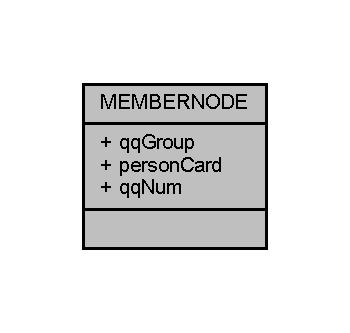
\includegraphics[width=168pt]{struct_m_e_m_b_e_r_n_o_d_e__coll__graph}
\end{center}
\end{figure}
\subsection*{Public 属性}
\begin{DoxyCompactItemize}
\item 
char \hyperlink{struct_m_e_m_b_e_r_n_o_d_e_a62b854a5f4fe02548468603da3796a3f}{qq\+Group} \mbox{[}100\mbox{]}
\item 
char \hyperlink{struct_m_e_m_b_e_r_n_o_d_e_aad1b94e7c25d824bb10accb1d12b4f77}{person\+Card} \mbox{[}100\mbox{]}
\item 
char \hyperlink{struct_m_e_m_b_e_r_n_o_d_e_a565763e23695fb0c7db2ccbb3e987ba0}{qq\+Num} \mbox{[}12\mbox{]}
\end{DoxyCompactItemize}


\subsection{详细描述}


在文件 Member\+Node.\+h 第 4 行定义.



\subsection{类成员变量说明}
\mbox{\Hypertarget{struct_m_e_m_b_e_r_n_o_d_e_aad1b94e7c25d824bb10accb1d12b4f77}\label{struct_m_e_m_b_e_r_n_o_d_e_aad1b94e7c25d824bb10accb1d12b4f77}} 
\index{M\+E\+M\+B\+E\+R\+N\+O\+DE@{M\+E\+M\+B\+E\+R\+N\+O\+DE}!person\+Card@{person\+Card}}
\index{person\+Card@{person\+Card}!M\+E\+M\+B\+E\+R\+N\+O\+DE@{M\+E\+M\+B\+E\+R\+N\+O\+DE}}
\subsubsection{\texorpdfstring{person\+Card}{personCard}}
{\footnotesize\ttfamily char M\+E\+M\+B\+E\+R\+N\+O\+D\+E\+::person\+Card\mbox{[}100\mbox{]}}



在文件 Member\+Node.\+h 第 7 行定义.

\mbox{\Hypertarget{struct_m_e_m_b_e_r_n_o_d_e_a62b854a5f4fe02548468603da3796a3f}\label{struct_m_e_m_b_e_r_n_o_d_e_a62b854a5f4fe02548468603da3796a3f}} 
\index{M\+E\+M\+B\+E\+R\+N\+O\+DE@{M\+E\+M\+B\+E\+R\+N\+O\+DE}!qq\+Group@{qq\+Group}}
\index{qq\+Group@{qq\+Group}!M\+E\+M\+B\+E\+R\+N\+O\+DE@{M\+E\+M\+B\+E\+R\+N\+O\+DE}}
\subsubsection{\texorpdfstring{qq\+Group}{qqGroup}}
{\footnotesize\ttfamily char M\+E\+M\+B\+E\+R\+N\+O\+D\+E\+::qq\+Group\mbox{[}100\mbox{]}}



在文件 Member\+Node.\+h 第 6 行定义.

\mbox{\Hypertarget{struct_m_e_m_b_e_r_n_o_d_e_a565763e23695fb0c7db2ccbb3e987ba0}\label{struct_m_e_m_b_e_r_n_o_d_e_a565763e23695fb0c7db2ccbb3e987ba0}} 
\index{M\+E\+M\+B\+E\+R\+N\+O\+DE@{M\+E\+M\+B\+E\+R\+N\+O\+DE}!qq\+Num@{qq\+Num}}
\index{qq\+Num@{qq\+Num}!M\+E\+M\+B\+E\+R\+N\+O\+DE@{M\+E\+M\+B\+E\+R\+N\+O\+DE}}
\subsubsection{\texorpdfstring{qq\+Num}{qqNum}}
{\footnotesize\ttfamily char M\+E\+M\+B\+E\+R\+N\+O\+D\+E\+::qq\+Num\mbox{[}12\mbox{]}}



在文件 Member\+Node.\+h 第 8 行定义.



该结构体的文档由以下文件生成\+:\begin{DoxyCompactItemize}
\item 
\hyperlink{_member_node_8h}{Member\+Node.\+h}\end{DoxyCompactItemize}

\hypertarget{struct_r_e_s_n_o_d_e}{}\section{R\+E\+S\+N\+O\+D\+E结构体 参考}
\label{struct_r_e_s_n_o_d_e}\index{R\+E\+S\+N\+O\+DE@{R\+E\+S\+N\+O\+DE}}


{\ttfamily \#include $<$res\+Node.\+h$>$}



R\+E\+S\+N\+O\+DE 的协作图\+:
\nopagebreak
\begin{figure}[H]
\begin{center}
\leavevmode
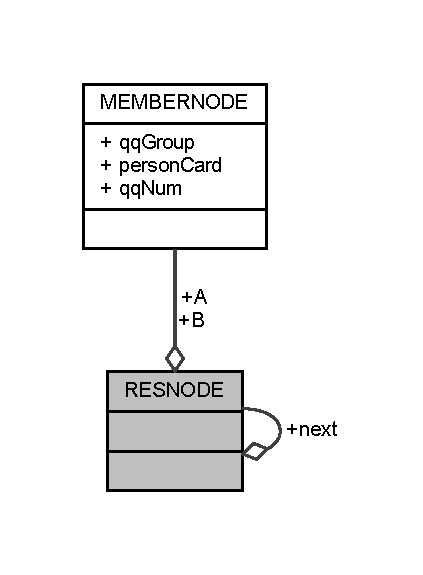
\includegraphics[width=203pt]{struct_r_e_s_n_o_d_e__coll__graph}
\end{center}
\end{figure}
\subsection*{Public 属性}
\begin{DoxyCompactItemize}
\item 
\hyperlink{_member_node_8h_af952c400512f5ff05a9356b68cb15730}{M\+N\+O\+DE} $\ast$ \hyperlink{struct_r_e_s_n_o_d_e_a51a4dc6b4f237be6b7668edec10f54c9}{A}
\item 
\hyperlink{_member_node_8h_af952c400512f5ff05a9356b68cb15730}{M\+N\+O\+DE} $\ast$ \hyperlink{struct_r_e_s_n_o_d_e_a7f54a8463ffa2e0e459aaf2de9beee47}{B}
\item 
struct \hyperlink{struct_r_e_s_n_o_d_e}{R\+E\+S\+N\+O\+DE} $\ast$ \hyperlink{struct_r_e_s_n_o_d_e_a76de7271a9ebedfb82e49bab978d3dd5}{next}
\end{DoxyCompactItemize}


\subsection{详细描述}


在文件 res\+Node.\+h 第 4 行定义.



\subsection{类成员变量说明}
\mbox{\Hypertarget{struct_r_e_s_n_o_d_e_a51a4dc6b4f237be6b7668edec10f54c9}\label{struct_r_e_s_n_o_d_e_a51a4dc6b4f237be6b7668edec10f54c9}} 
\index{R\+E\+S\+N\+O\+DE@{R\+E\+S\+N\+O\+DE}!A@{A}}
\index{A@{A}!R\+E\+S\+N\+O\+DE@{R\+E\+S\+N\+O\+DE}}
\subsubsection{\texorpdfstring{A}{A}}
{\footnotesize\ttfamily \hyperlink{_member_node_8h_af952c400512f5ff05a9356b68cb15730}{M\+N\+O\+DE}$\ast$ R\+E\+S\+N\+O\+D\+E\+::A}



在文件 res\+Node.\+h 第 6 行定义.

\mbox{\Hypertarget{struct_r_e_s_n_o_d_e_a7f54a8463ffa2e0e459aaf2de9beee47}\label{struct_r_e_s_n_o_d_e_a7f54a8463ffa2e0e459aaf2de9beee47}} 
\index{R\+E\+S\+N\+O\+DE@{R\+E\+S\+N\+O\+DE}!B@{B}}
\index{B@{B}!R\+E\+S\+N\+O\+DE@{R\+E\+S\+N\+O\+DE}}
\subsubsection{\texorpdfstring{B}{B}}
{\footnotesize\ttfamily \hyperlink{_member_node_8h_af952c400512f5ff05a9356b68cb15730}{M\+N\+O\+DE}$\ast$ R\+E\+S\+N\+O\+D\+E\+::B}



在文件 res\+Node.\+h 第 7 行定义.

\mbox{\Hypertarget{struct_r_e_s_n_o_d_e_a76de7271a9ebedfb82e49bab978d3dd5}\label{struct_r_e_s_n_o_d_e_a76de7271a9ebedfb82e49bab978d3dd5}} 
\index{R\+E\+S\+N\+O\+DE@{R\+E\+S\+N\+O\+DE}!next@{next}}
\index{next@{next}!R\+E\+S\+N\+O\+DE@{R\+E\+S\+N\+O\+DE}}
\subsubsection{\texorpdfstring{next}{next}}
{\footnotesize\ttfamily struct \hyperlink{struct_r_e_s_n_o_d_e}{R\+E\+S\+N\+O\+DE}$\ast$ R\+E\+S\+N\+O\+D\+E\+::next}



在文件 res\+Node.\+h 第 8 行定义.



该结构体的文档由以下文件生成\+:\begin{DoxyCompactItemize}
\item 
\hyperlink{res_node_8h}{res\+Node.\+h}\end{DoxyCompactItemize}

\hypertarget{struct_s_t_a_c_k_n_o_d_e}{}\section{S\+T\+A\+C\+K\+N\+O\+D\+E结构体 参考}
\label{struct_s_t_a_c_k_n_o_d_e}\index{S\+T\+A\+C\+K\+N\+O\+DE@{S\+T\+A\+C\+K\+N\+O\+DE}}


{\ttfamily \#include $<$S\+T\+A\+C\+K\+N\+O\+D\+E.\+h$>$}



S\+T\+A\+C\+K\+N\+O\+DE 的协作图\+:
\nopagebreak
\begin{figure}[H]
\begin{center}
\leavevmode
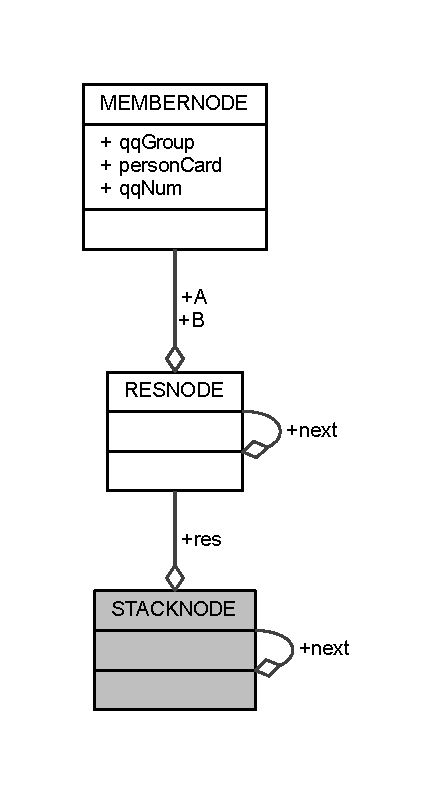
\includegraphics[width=209pt]{struct_s_t_a_c_k_n_o_d_e__coll__graph}
\end{center}
\end{figure}
\subsection*{Public 属性}
\begin{DoxyCompactItemize}
\item 
\hyperlink{res_node_8h_a99a496180780a83679ea667c9bc79fec}{res\+N\+O\+DE} $\ast$ \hyperlink{struct_s_t_a_c_k_n_o_d_e_afbbdf65611e982f361a73587b22aa862}{res}
\item 
struct \hyperlink{struct_s_t_a_c_k_n_o_d_e}{S\+T\+A\+C\+K\+N\+O\+DE} $\ast$ \hyperlink{struct_s_t_a_c_k_n_o_d_e_a50a11b6592f7f4903de61e4883bd7e34}{next}
\end{DoxyCompactItemize}


\subsection{详细描述}


在文件 S\+T\+A\+C\+K\+N\+O\+D\+E.\+h 第 3 行定义.



\subsection{类成员变量说明}
\mbox{\Hypertarget{struct_s_t_a_c_k_n_o_d_e_a50a11b6592f7f4903de61e4883bd7e34}\label{struct_s_t_a_c_k_n_o_d_e_a50a11b6592f7f4903de61e4883bd7e34}} 
\index{S\+T\+A\+C\+K\+N\+O\+DE@{S\+T\+A\+C\+K\+N\+O\+DE}!next@{next}}
\index{next@{next}!S\+T\+A\+C\+K\+N\+O\+DE@{S\+T\+A\+C\+K\+N\+O\+DE}}
\subsubsection{\texorpdfstring{next}{next}}
{\footnotesize\ttfamily struct \hyperlink{struct_s_t_a_c_k_n_o_d_e}{S\+T\+A\+C\+K\+N\+O\+DE}$\ast$ S\+T\+A\+C\+K\+N\+O\+D\+E\+::next}



在文件 S\+T\+A\+C\+K\+N\+O\+D\+E.\+h 第 6 行定义.

\mbox{\Hypertarget{struct_s_t_a_c_k_n_o_d_e_afbbdf65611e982f361a73587b22aa862}\label{struct_s_t_a_c_k_n_o_d_e_afbbdf65611e982f361a73587b22aa862}} 
\index{S\+T\+A\+C\+K\+N\+O\+DE@{S\+T\+A\+C\+K\+N\+O\+DE}!res@{res}}
\index{res@{res}!S\+T\+A\+C\+K\+N\+O\+DE@{S\+T\+A\+C\+K\+N\+O\+DE}}
\subsubsection{\texorpdfstring{res}{res}}
{\footnotesize\ttfamily \hyperlink{res_node_8h_a99a496180780a83679ea667c9bc79fec}{res\+N\+O\+DE}$\ast$ S\+T\+A\+C\+K\+N\+O\+D\+E\+::res}



在文件 S\+T\+A\+C\+K\+N\+O\+D\+E.\+h 第 5 行定义.



该结构体的文档由以下文件生成\+:\begin{DoxyCompactItemize}
\item 
\hyperlink{_s_t_a_c_k_n_o_d_e_8h}{S\+T\+A\+C\+K\+N\+O\+D\+E.\+h}\end{DoxyCompactItemize}

\chapter{文件说明}
\hypertarget{_b_i_n_node_8h}{}\section{B\+I\+N\+Node.\+h 文件参考}
\label{_b_i_n_node_8h}\index{B\+I\+N\+Node.\+h@{B\+I\+N\+Node.\+h}}
此图展示该文件直接或间接的被哪些文件引用了\+:
\nopagebreak
\begin{figure}[H]
\begin{center}
\leavevmode
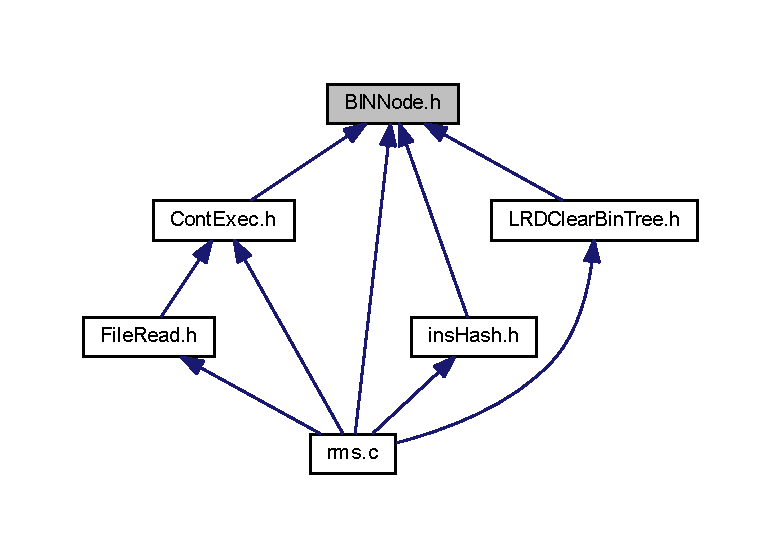
\includegraphics[width=350pt]{_b_i_n_node_8h__dep__incl}
\end{center}
\end{figure}
\subsection*{类}
\begin{DoxyCompactItemize}
\item 
struct \hyperlink{struct_b_i_n_t_r_e_e}{B\+I\+N\+T\+R\+EE}
\end{DoxyCompactItemize}
\subsection*{类型定义}
\begin{DoxyCompactItemize}
\item 
typedef struct \hyperlink{struct_b_i_n_t_r_e_e}{B\+I\+N\+T\+R\+EE} \hyperlink{_b_i_n_node_8h_a2fdaf7327a729b00aa89b6f5e3d6d336}{bin\+Tree\+N\+O\+DE}
\end{DoxyCompactItemize}


\subsection{类型定义说明}
\mbox{\Hypertarget{_b_i_n_node_8h_a2fdaf7327a729b00aa89b6f5e3d6d336}\label{_b_i_n_node_8h_a2fdaf7327a729b00aa89b6f5e3d6d336}} 
\index{B\+I\+N\+Node.\+h@{B\+I\+N\+Node.\+h}!bin\+Tree\+N\+O\+DE@{bin\+Tree\+N\+O\+DE}}
\index{bin\+Tree\+N\+O\+DE@{bin\+Tree\+N\+O\+DE}!B\+I\+N\+Node.\+h@{B\+I\+N\+Node.\+h}}
\subsubsection{\texorpdfstring{bin\+Tree\+N\+O\+DE}{binTreeNODE}}
{\footnotesize\ttfamily typedef struct \hyperlink{struct_b_i_n_t_r_e_e}{B\+I\+N\+T\+R\+EE} \hyperlink{_b_i_n_node_8h_a2fdaf7327a729b00aa89b6f5e3d6d336}{bin\+Tree\+N\+O\+DE}}


\hypertarget{_clear_hash_8h}{}\section{Clear\+Hash.\+h 文件参考}
\label{_clear_hash_8h}\index{Clear\+Hash.\+h@{Clear\+Hash.\+h}}
此图展示该文件直接或间接的被哪些文件引用了\+:
\nopagebreak
\begin{figure}[H]
\begin{center}
\leavevmode
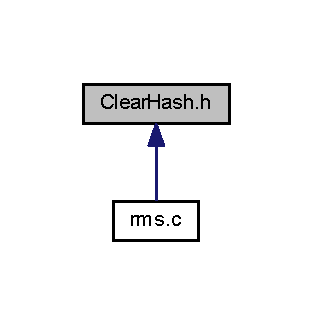
\includegraphics[width=150pt]{_clear_hash_8h__dep__incl}
\end{center}
\end{figure}
\subsection*{函数}
\begin{DoxyCompactItemize}
\item 
int \hyperlink{_clear_hash_8h_ac37a7ef6fdbfac0b41fc0244d7f09d6f}{Clear\+Hash} (\hyperlink{_b_i_n_node_8h_a2fdaf7327a729b00aa89b6f5e3d6d336}{bin\+Tree\+N\+O\+DE} $\ast$hash\mbox{[}$\,$\mbox{]})
\end{DoxyCompactItemize}


\subsection{函数说明}
\mbox{\Hypertarget{_clear_hash_8h_ac37a7ef6fdbfac0b41fc0244d7f09d6f}\label{_clear_hash_8h_ac37a7ef6fdbfac0b41fc0244d7f09d6f}} 
\index{Clear\+Hash.\+h@{Clear\+Hash.\+h}!Clear\+Hash@{Clear\+Hash}}
\index{Clear\+Hash@{Clear\+Hash}!Clear\+Hash.\+h@{Clear\+Hash.\+h}}
\subsubsection{\texorpdfstring{Clear\+Hash()}{ClearHash()}}
{\footnotesize\ttfamily int Clear\+Hash (\begin{DoxyParamCaption}\item[{\hyperlink{_b_i_n_node_8h_a2fdaf7327a729b00aa89b6f5e3d6d336}{bin\+Tree\+N\+O\+DE} $\ast$}]{hash\mbox{[}$\,$\mbox{]} }\end{DoxyParamCaption})}



在文件 Clear\+Hash.\+h 第 3 行定义.

这是这个函数的调用关系图\+:
\nopagebreak
\begin{figure}[H]
\begin{center}
\leavevmode
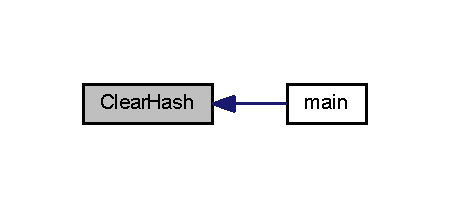
\includegraphics[width=216pt]{_clear_hash_8h_ac37a7ef6fdbfac0b41fc0244d7f09d6f_icgraph}
\end{center}
\end{figure}

\hypertarget{_clear_res_list_8h}{}\section{Clear\+Res\+List.\+h 文件参考}
\label{_clear_res_list_8h}\index{Clear\+Res\+List.\+h@{Clear\+Res\+List.\+h}}
此图展示该文件直接或间接的被哪些文件引用了\+:
\nopagebreak
\begin{figure}[H]
\begin{center}
\leavevmode
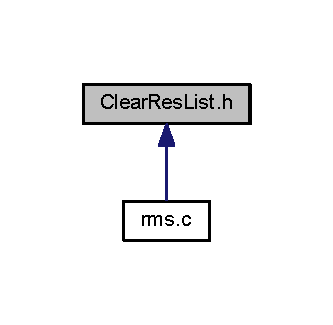
\includegraphics[width=160pt]{_clear_res_list_8h__dep__incl}
\end{center}
\end{figure}
\subsection*{函数}
\begin{DoxyCompactItemize}
\item 
int \hyperlink{_clear_res_list_8h_a766846d85a6013094ebf80cd7dd5589a}{Clear\+Res\+List} (\hyperlink{res_node_8h_a99a496180780a83679ea667c9bc79fec}{res\+N\+O\+DE} $\ast$list)
\end{DoxyCompactItemize}


\subsection{函数说明}
\mbox{\Hypertarget{_clear_res_list_8h_a766846d85a6013094ebf80cd7dd5589a}\label{_clear_res_list_8h_a766846d85a6013094ebf80cd7dd5589a}} 
\index{Clear\+Res\+List.\+h@{Clear\+Res\+List.\+h}!Clear\+Res\+List@{Clear\+Res\+List}}
\index{Clear\+Res\+List@{Clear\+Res\+List}!Clear\+Res\+List.\+h@{Clear\+Res\+List.\+h}}
\subsubsection{\texorpdfstring{Clear\+Res\+List()}{ClearResList()}}
{\footnotesize\ttfamily int Clear\+Res\+List (\begin{DoxyParamCaption}\item[{\hyperlink{res_node_8h_a99a496180780a83679ea667c9bc79fec}{res\+N\+O\+DE} $\ast$}]{list }\end{DoxyParamCaption})}



在文件 Clear\+Res\+List.\+h 第 3 行定义.

这是这个函数的调用关系图\+:
\nopagebreak
\begin{figure}[H]
\begin{center}
\leavevmode
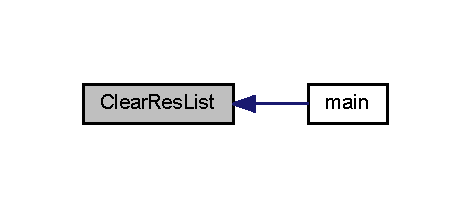
\includegraphics[width=226pt]{_clear_res_list_8h_a766846d85a6013094ebf80cd7dd5589a_icgraph}
\end{center}
\end{figure}

\hypertarget{_cont_exec_8h}{}\section{Cont\+Exec.\+h 文件参考}
\label{_cont_exec_8h}\index{Cont\+Exec.\+h@{Cont\+Exec.\+h}}
{\ttfamily \#include $<$malloc.\+h$>$}\newline
{\ttfamily \#include \char`\"{}B\+I\+N\+Node.\+h\char`\"{}}\newline
{\ttfamily \#include \char`\"{}Member\+Node.\+h\char`\"{}}\newline
Cont\+Exec.\+h 的引用(Include)关系图\+:
\nopagebreak
\begin{figure}[H]
\begin{center}
\leavevmode
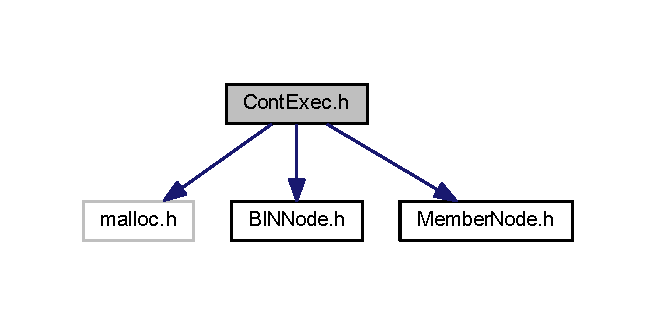
\includegraphics[width=315pt]{_cont_exec_8h__incl}
\end{center}
\end{figure}
此图展示该文件直接或间接的被哪些文件引用了\+:
\nopagebreak
\begin{figure}[H]
\begin{center}
\leavevmode
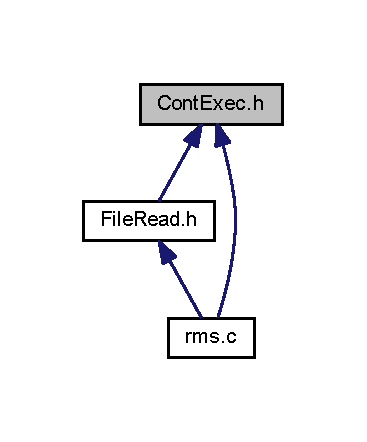
\includegraphics[width=176pt]{_cont_exec_8h__dep__incl}
\end{center}
\end{figure}
\subsection*{宏定义}
\begin{DoxyCompactItemize}
\item 
\#define \hyperlink{_cont_exec_8h_aba51915c87d64af47fb1cc59348961c9}{OK}~1
\item 
\#define \hyperlink{_cont_exec_8h_a735563036dced0b7d6cc98f97ea4978b}{E\+RR}~-\/1
\end{DoxyCompactItemize}
\subsection*{函数}
\begin{DoxyCompactItemize}
\item 
int \hyperlink{_cont_exec_8h_ab87770a1ba799e6e9a47c634f9d9000d}{contexec} (char $\ast$str, \hyperlink{_b_i_n_node_8h_a2fdaf7327a729b00aa89b6f5e3d6d336}{bin\+Tree\+N\+O\+DE} $\ast$hashT\mbox{[}$\,$\mbox{]})
\end{DoxyCompactItemize}


\subsection{宏定义说明}
\mbox{\Hypertarget{_cont_exec_8h_a735563036dced0b7d6cc98f97ea4978b}\label{_cont_exec_8h_a735563036dced0b7d6cc98f97ea4978b}} 
\index{Cont\+Exec.\+h@{Cont\+Exec.\+h}!E\+RR@{E\+RR}}
\index{E\+RR@{E\+RR}!Cont\+Exec.\+h@{Cont\+Exec.\+h}}
\subsubsection{\texorpdfstring{E\+RR}{ERR}}
{\footnotesize\ttfamily \#define E\+RR~-\/1}



在文件 Cont\+Exec.\+h 第 9 行定义.

\mbox{\Hypertarget{_cont_exec_8h_aba51915c87d64af47fb1cc59348961c9}\label{_cont_exec_8h_aba51915c87d64af47fb1cc59348961c9}} 
\index{Cont\+Exec.\+h@{Cont\+Exec.\+h}!OK@{OK}}
\index{OK@{OK}!Cont\+Exec.\+h@{Cont\+Exec.\+h}}
\subsubsection{\texorpdfstring{OK}{OK}}
{\footnotesize\ttfamily \#define OK~1}



在文件 Cont\+Exec.\+h 第 8 行定义.



\subsection{函数说明}
\mbox{\Hypertarget{_cont_exec_8h_ab87770a1ba799e6e9a47c634f9d9000d}\label{_cont_exec_8h_ab87770a1ba799e6e9a47c634f9d9000d}} 
\index{Cont\+Exec.\+h@{Cont\+Exec.\+h}!contexec@{contexec}}
\index{contexec@{contexec}!Cont\+Exec.\+h@{Cont\+Exec.\+h}}
\subsubsection{\texorpdfstring{contexec()}{contexec()}}
{\footnotesize\ttfamily int contexec (\begin{DoxyParamCaption}\item[{char $\ast$}]{str,  }\item[{\hyperlink{_b_i_n_node_8h_a2fdaf7327a729b00aa89b6f5e3d6d336}{bin\+Tree\+N\+O\+DE} $\ast$}]{hashT\mbox{[}$\,$\mbox{]} }\end{DoxyParamCaption})}



在文件 Cont\+Exec.\+h 第 16 行定义.

函数调用图\+:
\nopagebreak
\begin{figure}[H]
\begin{center}
\leavevmode
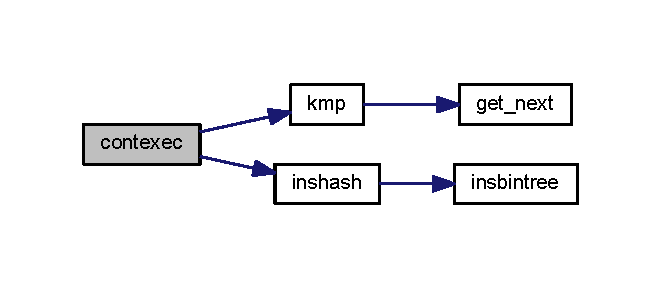
\includegraphics[width=317pt]{_cont_exec_8h_ab87770a1ba799e6e9a47c634f9d9000d_cgraph}
\end{center}
\end{figure}
这是这个函数的调用关系图\+:
\nopagebreak
\begin{figure}[H]
\begin{center}
\leavevmode
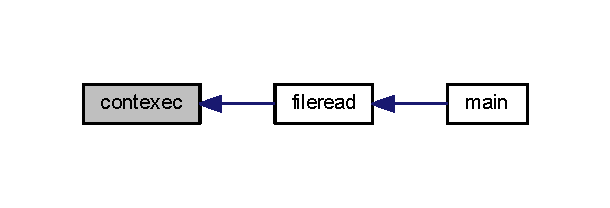
\includegraphics[width=293pt]{_cont_exec_8h_ab87770a1ba799e6e9a47c634f9d9000d_icgraph}
\end{center}
\end{figure}

\hypertarget{_d_l_r_search_bin_tree_8h}{}\section{D\+L\+R\+Search\+Bin\+Tree.\+h 文件参考}
\label{_d_l_r_search_bin_tree_8h}\index{D\+L\+R\+Search\+Bin\+Tree.\+h@{D\+L\+R\+Search\+Bin\+Tree.\+h}}
此图展示该文件直接或间接的被哪些文件引用了\+:
\nopagebreak
\begin{figure}[H]
\begin{center}
\leavevmode
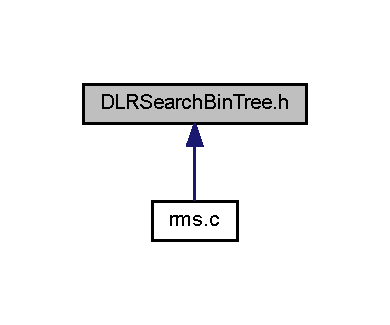
\includegraphics[width=187pt]{_d_l_r_search_bin_tree_8h__dep__incl}
\end{center}
\end{figure}
\subsection*{函数}
\begin{DoxyCompactItemize}
\item 
int \hyperlink{_d_l_r_search_bin_tree_8h_aa72f933e3e298f2af320242baed64df3}{D\+L\+Rsearchbintree} (\hyperlink{_b_i_n_node_8h_a2fdaf7327a729b00aa89b6f5e3d6d336}{bin\+Tree\+N\+O\+DE} $\ast$bintree, \hyperlink{_b_i_n_node_8h_a2fdaf7327a729b00aa89b6f5e3d6d336}{bin\+Tree\+N\+O\+DE} $\ast$item, \hyperlink{res_node_8h_a99a496180780a83679ea667c9bc79fec}{res\+N\+O\+DE} $\ast$res\+List)
\end{DoxyCompactItemize}


\subsection{函数说明}
\mbox{\Hypertarget{_d_l_r_search_bin_tree_8h_aa72f933e3e298f2af320242baed64df3}\label{_d_l_r_search_bin_tree_8h_aa72f933e3e298f2af320242baed64df3}} 
\index{D\+L\+R\+Search\+Bin\+Tree.\+h@{D\+L\+R\+Search\+Bin\+Tree.\+h}!D\+L\+Rsearchbintree@{D\+L\+Rsearchbintree}}
\index{D\+L\+Rsearchbintree@{D\+L\+Rsearchbintree}!D\+L\+R\+Search\+Bin\+Tree.\+h@{D\+L\+R\+Search\+Bin\+Tree.\+h}}
\subsubsection{\texorpdfstring{D\+L\+Rsearchbintree()}{DLRsearchbintree()}}
{\footnotesize\ttfamily int D\+L\+Rsearchbintree (\begin{DoxyParamCaption}\item[{\hyperlink{_b_i_n_node_8h_a2fdaf7327a729b00aa89b6f5e3d6d336}{bin\+Tree\+N\+O\+DE} $\ast$}]{bintree,  }\item[{\hyperlink{_b_i_n_node_8h_a2fdaf7327a729b00aa89b6f5e3d6d336}{bin\+Tree\+N\+O\+DE} $\ast$}]{item,  }\item[{\hyperlink{res_node_8h_a99a496180780a83679ea667c9bc79fec}{res\+N\+O\+DE} $\ast$}]{res\+List }\end{DoxyParamCaption})}



在文件 D\+L\+R\+Search\+Bin\+Tree.\+h 第 4 行定义.

函数调用图\+:
\nopagebreak
\begin{figure}[H]
\begin{center}
\leavevmode
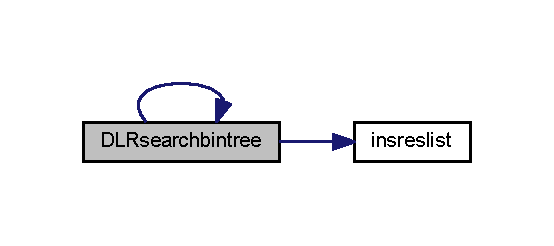
\includegraphics[width=266pt]{_d_l_r_search_bin_tree_8h_aa72f933e3e298f2af320242baed64df3_cgraph}
\end{center}
\end{figure}
这是这个函数的调用关系图\+:
\nopagebreak
\begin{figure}[H]
\begin{center}
\leavevmode
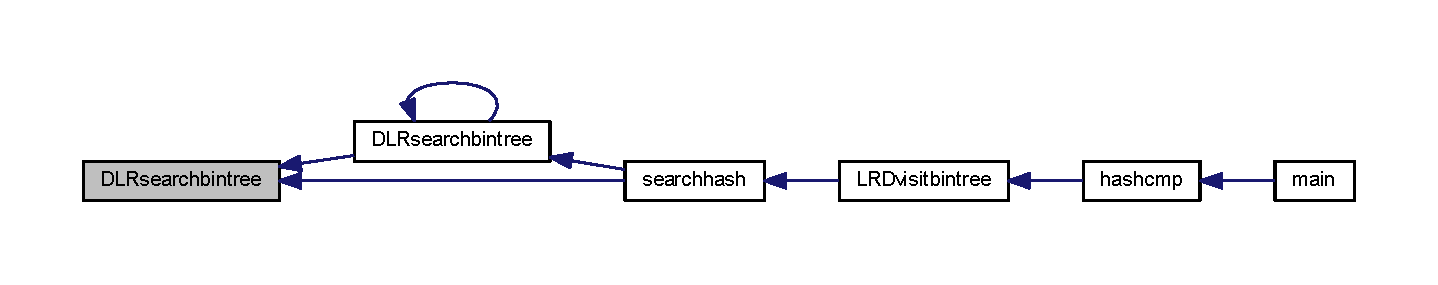
\includegraphics[width=350pt]{_d_l_r_search_bin_tree_8h_aa72f933e3e298f2af320242baed64df3_icgraph}
\end{center}
\end{figure}

\hypertarget{_file_read_8h}{}\section{File\+Read.\+h 文件参考}
\label{_file_read_8h}\index{File\+Read.\+h@{File\+Read.\+h}}
{\ttfamily \#include $<$stdio.\+h$>$}\newline
{\ttfamily \#include \char`\"{}Cont\+Exec.\+h\char`\"{}}\newline
File\+Read.\+h 的引用(Include)关系图\+:
\nopagebreak
\begin{figure}[H]
\begin{center}
\leavevmode
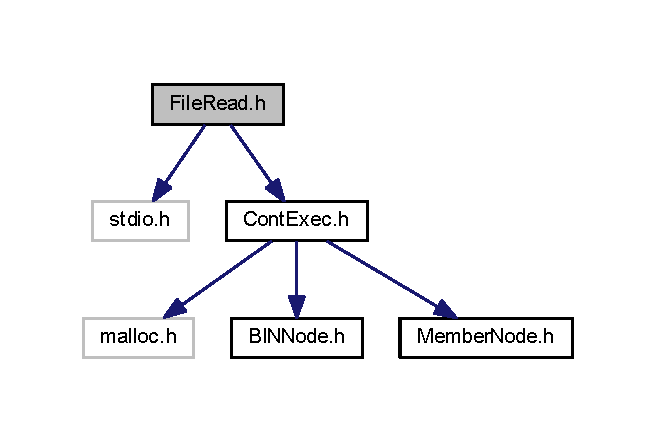
\includegraphics[width=315pt]{_file_read_8h__incl}
\end{center}
\end{figure}
此图展示该文件直接或间接的被哪些文件引用了\+:
\nopagebreak
\begin{figure}[H]
\begin{center}
\leavevmode
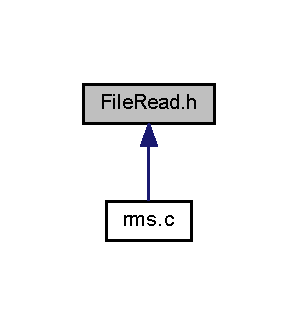
\includegraphics[width=143pt]{_file_read_8h__dep__incl}
\end{center}
\end{figure}
\subsection*{函数}
\begin{DoxyCompactItemize}
\item 
int \hyperlink{_file_read_8h_ad17368ccbe75d3a2a856199391c226c3}{fileread} (char $\ast$url, \hyperlink{_b_i_n_node_8h_a2fdaf7327a729b00aa89b6f5e3d6d336}{bin\+Tree\+N\+O\+DE} $\ast$hash\mbox{[}$\,$\mbox{]})
\end{DoxyCompactItemize}


\subsection{函数说明}
\mbox{\Hypertarget{_file_read_8h_ad17368ccbe75d3a2a856199391c226c3}\label{_file_read_8h_ad17368ccbe75d3a2a856199391c226c3}} 
\index{File\+Read.\+h@{File\+Read.\+h}!fileread@{fileread}}
\index{fileread@{fileread}!File\+Read.\+h@{File\+Read.\+h}}
\subsubsection{\texorpdfstring{fileread()}{fileread()}}
{\footnotesize\ttfamily int fileread (\begin{DoxyParamCaption}\item[{char $\ast$}]{url,  }\item[{\hyperlink{_b_i_n_node_8h_a2fdaf7327a729b00aa89b6f5e3d6d336}{bin\+Tree\+N\+O\+DE} $\ast$}]{hash\mbox{[}$\,$\mbox{]} }\end{DoxyParamCaption})}



在文件 File\+Read.\+h 第 9 行定义.

函数调用图\+:
\nopagebreak
\begin{figure}[H]
\begin{center}
\leavevmode
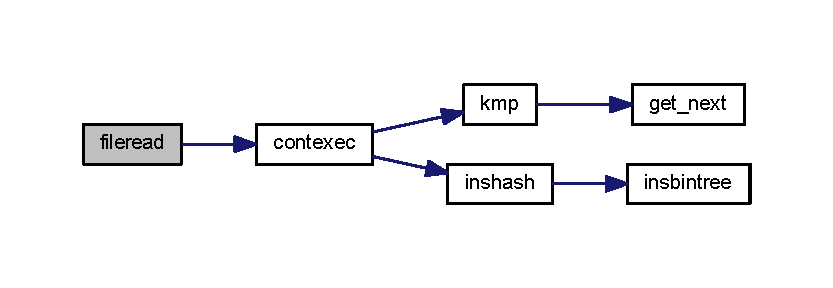
\includegraphics[width=350pt]{_file_read_8h_ad17368ccbe75d3a2a856199391c226c3_cgraph}
\end{center}
\end{figure}
这是这个函数的调用关系图\+:
\nopagebreak
\begin{figure}[H]
\begin{center}
\leavevmode
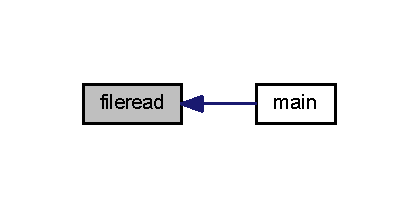
\includegraphics[width=201pt]{_file_read_8h_ad17368ccbe75d3a2a856199391c226c3_icgraph}
\end{center}
\end{figure}

\hypertarget{_file_write_8h}{}\section{File\+Write.\+h 文件参考}
\label{_file_write_8h}\index{File\+Write.\+h@{File\+Write.\+h}}
{\ttfamily \#include $<$stdio.\+h$>$}\newline
File\+Write.\+h 的引用(Include)关系图\+:
\nopagebreak
\begin{figure}[H]
\begin{center}
\leavevmode
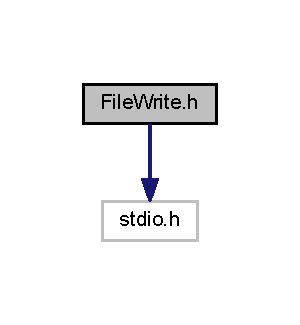
\includegraphics[width=144pt]{_file_write_8h__incl}
\end{center}
\end{figure}
此图展示该文件直接或间接的被哪些文件引用了\+:
\nopagebreak
\begin{figure}[H]
\begin{center}
\leavevmode
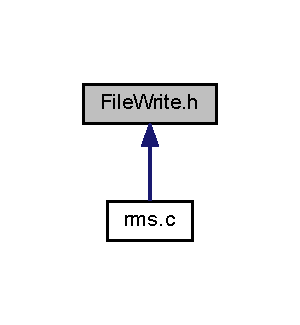
\includegraphics[width=144pt]{_file_write_8h__dep__incl}
\end{center}
\end{figure}
\subsection*{函数}
\begin{DoxyCompactItemize}
\item 
int \hyperlink{_file_write_8h_a2c87ece9636bca846c34c22ad8f81607}{File\+Write} (\hyperlink{res_node_8h_a99a496180780a83679ea667c9bc79fec}{res\+N\+O\+DE} $\ast$list, char $\ast$filename)
\end{DoxyCompactItemize}


\subsection{函数说明}
\mbox{\Hypertarget{_file_write_8h_a2c87ece9636bca846c34c22ad8f81607}\label{_file_write_8h_a2c87ece9636bca846c34c22ad8f81607}} 
\index{File\+Write.\+h@{File\+Write.\+h}!File\+Write@{File\+Write}}
\index{File\+Write@{File\+Write}!File\+Write.\+h@{File\+Write.\+h}}
\subsubsection{\texorpdfstring{File\+Write()}{FileWrite()}}
{\footnotesize\ttfamily int File\+Write (\begin{DoxyParamCaption}\item[{\hyperlink{res_node_8h_a99a496180780a83679ea667c9bc79fec}{res\+N\+O\+DE} $\ast$}]{list,  }\item[{char $\ast$}]{filename }\end{DoxyParamCaption})}



在文件 File\+Write.\+h 第 4 行定义.

这是这个函数的调用关系图\+:
\nopagebreak
\begin{figure}[H]
\begin{center}
\leavevmode
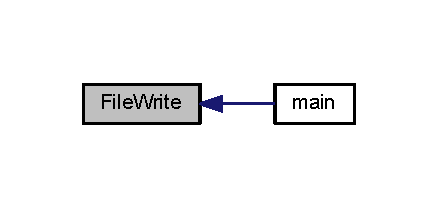
\includegraphics[width=210pt]{_file_write_8h_a2c87ece9636bca846c34c22ad8f81607_icgraph}
\end{center}
\end{figure}

\hypertarget{_function_8h}{}\section{Function.\+h 文件参考}
\label{_function_8h}\index{Function.\+h@{Function.\+h}}
此图展示该文件直接或间接的被哪些文件引用了\+:
\nopagebreak
\begin{figure}[H]
\begin{center}
\leavevmode
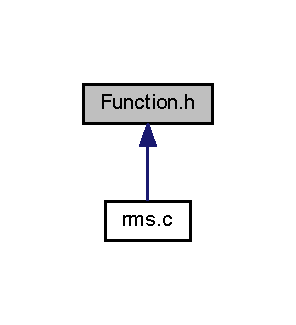
\includegraphics[width=142pt]{_function_8h__dep__incl}
\end{center}
\end{figure}
\subsection*{函数}
\begin{DoxyCompactItemize}
\item 
void \hyperlink{_function_8h_a1e3b6d38df0786ccf7f938d60e386aae}{Init} ()
\item 
int \hyperlink{_function_8h_a906a9068d36c3b9b81a504bdd5a05dc7}{fileread} (char $\ast$filename, \hyperlink{_b_i_n_node_8h_a2fdaf7327a729b00aa89b6f5e3d6d336}{bin\+Tree\+N\+O\+DE} $\ast$hash\mbox{[}$\,$\mbox{]})
\item 
int \hyperlink{_function_8h_ab87770a1ba799e6e9a47c634f9d9000d}{contexec} (char $\ast$str, \hyperlink{_b_i_n_node_8h_a2fdaf7327a729b00aa89b6f5e3d6d336}{bin\+Tree\+N\+O\+DE} $\ast$hashT\mbox{[}$\,$\mbox{]})
\item 
int \hyperlink{_function_8h_af78bb1b244bd36a7f9007b7f9648fd6a}{is\+Chinese} (char $\ast$)
\item 
long \hyperlink{_function_8h_ad40e7a9497ff7a575f32784f4887fc7c}{kmp} (char $\ast$master, char $\ast$pattern, long pos)
\item 
int \hyperlink{_function_8h_a3cb1827c44099e76fe08fe6e409445fa}{searchhash} (\hyperlink{_b_i_n_node_8h_a2fdaf7327a729b00aa89b6f5e3d6d336}{bin\+Tree\+N\+O\+DE} $\ast$bintree, \hyperlink{_b_i_n_node_8h_a2fdaf7327a729b00aa89b6f5e3d6d336}{bin\+Tree\+N\+O\+DE} $\ast$hashB\mbox{[}$\,$\mbox{]}, \hyperlink{res_node_8h_a99a496180780a83679ea667c9bc79fec}{res\+N\+O\+DE} $\ast$res\+List)
\item 
int \hyperlink{_function_8h_a1021ef2a4552ed9174ab6bd0f9e0b77a}{insreslist} (\hyperlink{res_node_8h_a99a496180780a83679ea667c9bc79fec}{res\+N\+O\+DE} $\ast$list, \hyperlink{res_node_8h_a99a496180780a83679ea667c9bc79fec}{res\+N\+O\+DE} $\ast$p)
\item 
int \hyperlink{_function_8h_ae3057c044e96d31c1b28f1308551acbb}{insbintree} (\hyperlink{_b_i_n_node_8h_a2fdaf7327a729b00aa89b6f5e3d6d336}{bin\+Tree\+N\+O\+DE} $\ast$, \hyperlink{_b_i_n_node_8h_a2fdaf7327a729b00aa89b6f5e3d6d336}{bin\+Tree\+N\+O\+DE} $\ast$)
\item 
int \hyperlink{_function_8h_a5a318354c875367310f84de442acee2e}{hashcmp} (\hyperlink{_b_i_n_node_8h_a2fdaf7327a729b00aa89b6f5e3d6d336}{bin\+Tree\+N\+O\+DE} $\ast$hashA\mbox{[}$\,$\mbox{]}, \hyperlink{_b_i_n_node_8h_a2fdaf7327a729b00aa89b6f5e3d6d336}{bin\+Tree\+N\+O\+DE} $\ast$hashB\mbox{[}$\,$\mbox{]}, \hyperlink{res_node_8h_a99a496180780a83679ea667c9bc79fec}{res\+N\+O\+DE} $\ast$res\+List)
\item 
int \hyperlink{_function_8h_a9164bd1b5c092f69060bdd4285f8917c}{L\+R\+Dvisitbintree} (\hyperlink{_b_i_n_node_8h_a2fdaf7327a729b00aa89b6f5e3d6d336}{bin\+Tree\+N\+O\+DE} $\ast$bintree, \hyperlink{_b_i_n_node_8h_a2fdaf7327a729b00aa89b6f5e3d6d336}{bin\+Tree\+N\+O\+DE} $\ast$hashB\mbox{[}$\,$\mbox{]}, \hyperlink{res_node_8h_a99a496180780a83679ea667c9bc79fec}{res\+N\+O\+DE} $\ast$res\+List)
\item 
int \hyperlink{_function_8h_aa72f933e3e298f2af320242baed64df3}{D\+L\+Rsearchbintree} (\hyperlink{_b_i_n_node_8h_a2fdaf7327a729b00aa89b6f5e3d6d336}{bin\+Tree\+N\+O\+DE} $\ast$bintree, \hyperlink{_b_i_n_node_8h_a2fdaf7327a729b00aa89b6f5e3d6d336}{bin\+Tree\+N\+O\+DE} $\ast$item, \hyperlink{res_node_8h_a99a496180780a83679ea667c9bc79fec}{res\+N\+O\+DE} $\ast$res\+List)
\item 
int \hyperlink{_function_8h_a2c87ece9636bca846c34c22ad8f81607}{File\+Write} (\hyperlink{res_node_8h_a99a496180780a83679ea667c9bc79fec}{res\+N\+O\+DE} $\ast$list, char $\ast$filename)
\item 
int \hyperlink{_function_8h_acb0a1c9171ae96f2076bffd6dfe752e3}{Quick\+Sort} (\hyperlink{res_node_8h_a99a496180780a83679ea667c9bc79fec}{res\+N\+O\+DE} $\ast$list, \hyperlink{res_node_8h_a99a496180780a83679ea667c9bc79fec}{res\+N\+O\+DE} $\ast$end)
\item 
int \hyperlink{_function_8h_a60c4ee271e18fa873ee5365cd50b8b53}{Push\+Stack} (\hyperlink{_s_t_a_c_k_n_o_d_e_8h_a29d53fde99d01064acfd82258fbc54d7}{S\+T\+A\+CK} $\ast$stack, \hyperlink{_s_t_a_c_k_n_o_d_e_8h_a29d53fde99d01064acfd82258fbc54d7}{S\+T\+A\+CK} $\ast$item)
\item 
\hyperlink{_s_t_a_c_k_n_o_d_e_8h_a29d53fde99d01064acfd82258fbc54d7}{S\+T\+A\+CK} $\ast$ \hyperlink{_function_8h_a10b2b9a305b4ff344a5018171901a661}{Pop\+Stack} (\hyperlink{_s_t_a_c_k_n_o_d_e_8h_a29d53fde99d01064acfd82258fbc54d7}{S\+T\+A\+CK} $\ast$stack)
\item 
void \hyperlink{_function_8h_a916d9eda097fba327f23e85b1af09821}{Show\+Result} (\hyperlink{res_node_8h_a99a496180780a83679ea667c9bc79fec}{res\+N\+O\+DE} $\ast$list)
\item 
int \hyperlink{_function_8h_a766846d85a6013094ebf80cd7dd5589a}{Clear\+Res\+List} (\hyperlink{res_node_8h_a99a496180780a83679ea667c9bc79fec}{res\+N\+O\+DE} $\ast$list)
\item 
int \hyperlink{_function_8h_ac37a7ef6fdbfac0b41fc0244d7f09d6f}{Clear\+Hash} (\hyperlink{_b_i_n_node_8h_a2fdaf7327a729b00aa89b6f5e3d6d336}{bin\+Tree\+N\+O\+DE} $\ast$hash\mbox{[}$\,$\mbox{]})
\item 
int \hyperlink{_function_8h_a98ae0a41ca54ee951b33e6561dd0572b}{L\+R\+D\+Clear\+Bin\+Tree} (\hyperlink{_b_i_n_node_8h_a2fdaf7327a729b00aa89b6f5e3d6d336}{bin\+Tree\+N\+O\+DE} $\ast$bintree)
\item 
int \hyperlink{_function_8h_a7178f51f223e60c091b7c765abeba469}{inshash} (\hyperlink{_b_i_n_node_8h_a2fdaf7327a729b00aa89b6f5e3d6d336}{bin\+Tree\+N\+O\+DE} $\ast$hashT\mbox{[}$\,$\mbox{]}, \hyperlink{_b_i_n_node_8h_a2fdaf7327a729b00aa89b6f5e3d6d336}{bin\+Tree\+N\+O\+DE} $\ast$item)
\end{DoxyCompactItemize}


\subsection{函数说明}
\mbox{\Hypertarget{_function_8h_ac37a7ef6fdbfac0b41fc0244d7f09d6f}\label{_function_8h_ac37a7ef6fdbfac0b41fc0244d7f09d6f}} 
\index{Function.\+h@{Function.\+h}!Clear\+Hash@{Clear\+Hash}}
\index{Clear\+Hash@{Clear\+Hash}!Function.\+h@{Function.\+h}}
\subsubsection{\texorpdfstring{Clear\+Hash()}{ClearHash()}}
{\footnotesize\ttfamily int Clear\+Hash (\begin{DoxyParamCaption}\item[{\hyperlink{_b_i_n_node_8h_a2fdaf7327a729b00aa89b6f5e3d6d336}{bin\+Tree\+N\+O\+DE} $\ast$}]{hash\mbox{[}$\,$\mbox{]} }\end{DoxyParamCaption})}



在文件 Clear\+Hash.\+h 第 3 行定义.

这是这个函数的调用关系图\+:
\nopagebreak
\begin{figure}[H]
\begin{center}
\leavevmode
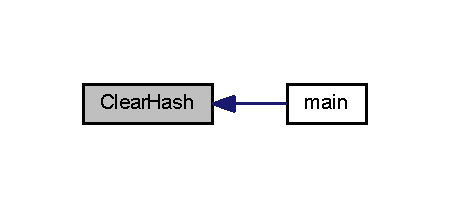
\includegraphics[width=216pt]{_function_8h_ac37a7ef6fdbfac0b41fc0244d7f09d6f_icgraph}
\end{center}
\end{figure}
\mbox{\Hypertarget{_function_8h_a766846d85a6013094ebf80cd7dd5589a}\label{_function_8h_a766846d85a6013094ebf80cd7dd5589a}} 
\index{Function.\+h@{Function.\+h}!Clear\+Res\+List@{Clear\+Res\+List}}
\index{Clear\+Res\+List@{Clear\+Res\+List}!Function.\+h@{Function.\+h}}
\subsubsection{\texorpdfstring{Clear\+Res\+List()}{ClearResList()}}
{\footnotesize\ttfamily int Clear\+Res\+List (\begin{DoxyParamCaption}\item[{\hyperlink{res_node_8h_a99a496180780a83679ea667c9bc79fec}{res\+N\+O\+DE} $\ast$}]{list }\end{DoxyParamCaption})}



在文件 Clear\+Res\+List.\+h 第 3 行定义.

这是这个函数的调用关系图\+:
\nopagebreak
\begin{figure}[H]
\begin{center}
\leavevmode
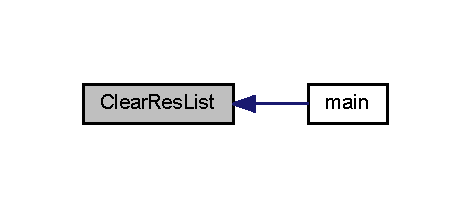
\includegraphics[width=226pt]{_function_8h_a766846d85a6013094ebf80cd7dd5589a_icgraph}
\end{center}
\end{figure}
\mbox{\Hypertarget{_function_8h_ab87770a1ba799e6e9a47c634f9d9000d}\label{_function_8h_ab87770a1ba799e6e9a47c634f9d9000d}} 
\index{Function.\+h@{Function.\+h}!contexec@{contexec}}
\index{contexec@{contexec}!Function.\+h@{Function.\+h}}
\subsubsection{\texorpdfstring{contexec()}{contexec()}}
{\footnotesize\ttfamily int contexec (\begin{DoxyParamCaption}\item[{char $\ast$}]{str,  }\item[{\hyperlink{_b_i_n_node_8h_a2fdaf7327a729b00aa89b6f5e3d6d336}{bin\+Tree\+N\+O\+DE} $\ast$}]{hashT\mbox{[}$\,$\mbox{]} }\end{DoxyParamCaption})}



在文件 Cont\+Exec.\+h 第 16 行定义.

函数调用图\+:
\nopagebreak
\begin{figure}[H]
\begin{center}
\leavevmode
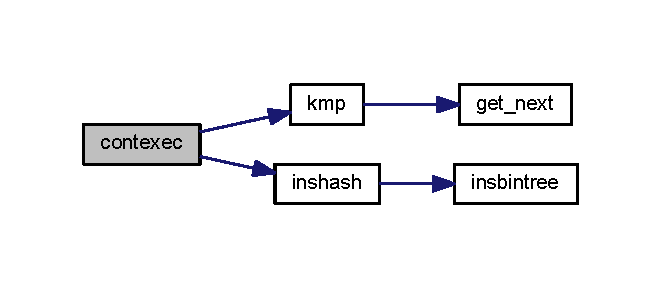
\includegraphics[width=317pt]{_function_8h_ab87770a1ba799e6e9a47c634f9d9000d_cgraph}
\end{center}
\end{figure}
这是这个函数的调用关系图\+:
\nopagebreak
\begin{figure}[H]
\begin{center}
\leavevmode
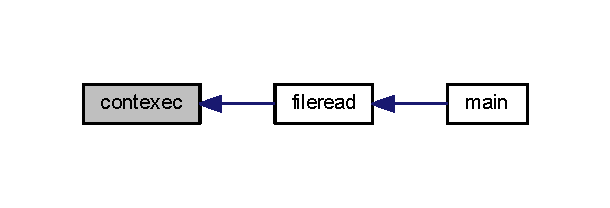
\includegraphics[width=293pt]{_function_8h_ab87770a1ba799e6e9a47c634f9d9000d_icgraph}
\end{center}
\end{figure}
\mbox{\Hypertarget{_function_8h_aa72f933e3e298f2af320242baed64df3}\label{_function_8h_aa72f933e3e298f2af320242baed64df3}} 
\index{Function.\+h@{Function.\+h}!D\+L\+Rsearchbintree@{D\+L\+Rsearchbintree}}
\index{D\+L\+Rsearchbintree@{D\+L\+Rsearchbintree}!Function.\+h@{Function.\+h}}
\subsubsection{\texorpdfstring{D\+L\+Rsearchbintree()}{DLRsearchbintree()}}
{\footnotesize\ttfamily int D\+L\+Rsearchbintree (\begin{DoxyParamCaption}\item[{\hyperlink{_b_i_n_node_8h_a2fdaf7327a729b00aa89b6f5e3d6d336}{bin\+Tree\+N\+O\+DE} $\ast$}]{bintree,  }\item[{\hyperlink{_b_i_n_node_8h_a2fdaf7327a729b00aa89b6f5e3d6d336}{bin\+Tree\+N\+O\+DE} $\ast$}]{item,  }\item[{\hyperlink{res_node_8h_a99a496180780a83679ea667c9bc79fec}{res\+N\+O\+DE} $\ast$}]{res\+List }\end{DoxyParamCaption})}



在文件 D\+L\+R\+Search\+Bin\+Tree.\+h 第 4 行定义.

函数调用图\+:
\nopagebreak
\begin{figure}[H]
\begin{center}
\leavevmode
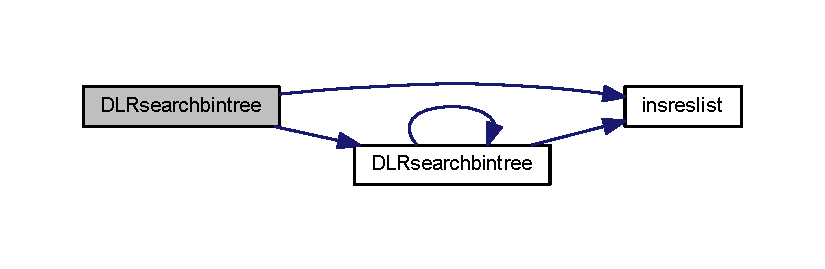
\includegraphics[width=350pt]{_function_8h_aa72f933e3e298f2af320242baed64df3_cgraph}
\end{center}
\end{figure}
这是这个函数的调用关系图\+:
\nopagebreak
\begin{figure}[H]
\begin{center}
\leavevmode
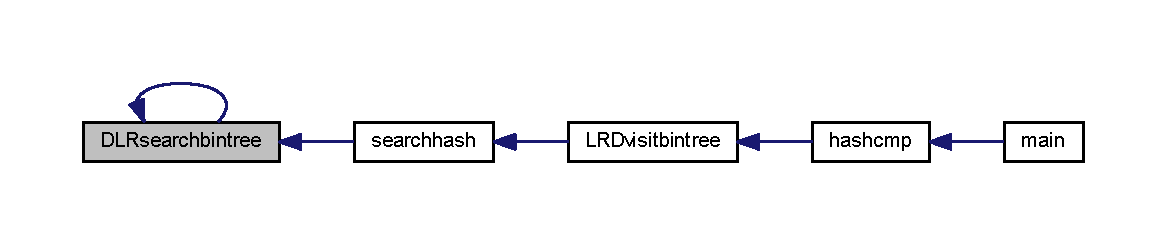
\includegraphics[width=350pt]{_function_8h_aa72f933e3e298f2af320242baed64df3_icgraph}
\end{center}
\end{figure}
\mbox{\Hypertarget{_function_8h_a906a9068d36c3b9b81a504bdd5a05dc7}\label{_function_8h_a906a9068d36c3b9b81a504bdd5a05dc7}} 
\index{Function.\+h@{Function.\+h}!fileread@{fileread}}
\index{fileread@{fileread}!Function.\+h@{Function.\+h}}
\subsubsection{\texorpdfstring{fileread()}{fileread()}}
{\footnotesize\ttfamily int fileread (\begin{DoxyParamCaption}\item[{char $\ast$}]{filename,  }\item[{\hyperlink{_b_i_n_node_8h_a2fdaf7327a729b00aa89b6f5e3d6d336}{bin\+Tree\+N\+O\+DE} $\ast$}]{hash\mbox{[}$\,$\mbox{]} }\end{DoxyParamCaption})}



在文件 File\+Read.\+h 第 9 行定义.

函数调用图\+:
\nopagebreak
\begin{figure}[H]
\begin{center}
\leavevmode
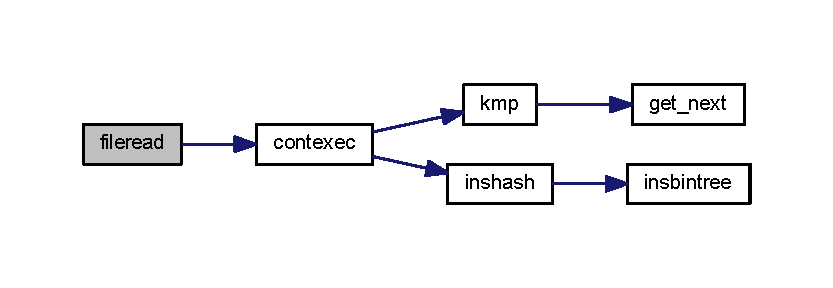
\includegraphics[width=350pt]{_function_8h_a906a9068d36c3b9b81a504bdd5a05dc7_cgraph}
\end{center}
\end{figure}
这是这个函数的调用关系图\+:
\nopagebreak
\begin{figure}[H]
\begin{center}
\leavevmode
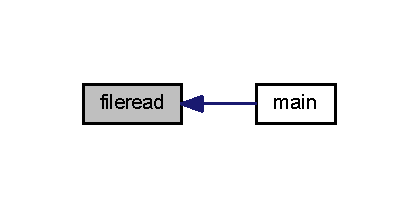
\includegraphics[width=201pt]{_function_8h_a906a9068d36c3b9b81a504bdd5a05dc7_icgraph}
\end{center}
\end{figure}
\mbox{\Hypertarget{_function_8h_a2c87ece9636bca846c34c22ad8f81607}\label{_function_8h_a2c87ece9636bca846c34c22ad8f81607}} 
\index{Function.\+h@{Function.\+h}!File\+Write@{File\+Write}}
\index{File\+Write@{File\+Write}!Function.\+h@{Function.\+h}}
\subsubsection{\texorpdfstring{File\+Write()}{FileWrite()}}
{\footnotesize\ttfamily int File\+Write (\begin{DoxyParamCaption}\item[{\hyperlink{res_node_8h_a99a496180780a83679ea667c9bc79fec}{res\+N\+O\+DE} $\ast$}]{list,  }\item[{char $\ast$}]{filename }\end{DoxyParamCaption})}



在文件 File\+Write.\+h 第 4 行定义.

这是这个函数的调用关系图\+:
\nopagebreak
\begin{figure}[H]
\begin{center}
\leavevmode
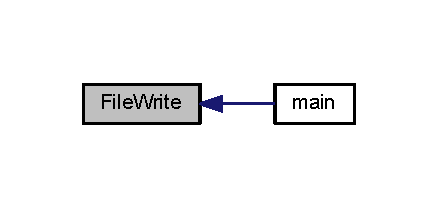
\includegraphics[width=210pt]{_function_8h_a2c87ece9636bca846c34c22ad8f81607_icgraph}
\end{center}
\end{figure}
\mbox{\Hypertarget{_function_8h_a5a318354c875367310f84de442acee2e}\label{_function_8h_a5a318354c875367310f84de442acee2e}} 
\index{Function.\+h@{Function.\+h}!hashcmp@{hashcmp}}
\index{hashcmp@{hashcmp}!Function.\+h@{Function.\+h}}
\subsubsection{\texorpdfstring{hashcmp()}{hashcmp()}}
{\footnotesize\ttfamily int hashcmp (\begin{DoxyParamCaption}\item[{\hyperlink{_b_i_n_node_8h_a2fdaf7327a729b00aa89b6f5e3d6d336}{bin\+Tree\+N\+O\+DE} $\ast$}]{hashA\mbox{[}$\,$\mbox{]},  }\item[{\hyperlink{_b_i_n_node_8h_a2fdaf7327a729b00aa89b6f5e3d6d336}{bin\+Tree\+N\+O\+DE} $\ast$}]{hashB\mbox{[}$\,$\mbox{]},  }\item[{\hyperlink{res_node_8h_a99a496180780a83679ea667c9bc79fec}{res\+N\+O\+DE} $\ast$}]{res\+List }\end{DoxyParamCaption})}



在文件 Hash\+Cmp.\+h 第 5 行定义.

函数调用图\+:
\nopagebreak
\begin{figure}[H]
\begin{center}
\leavevmode
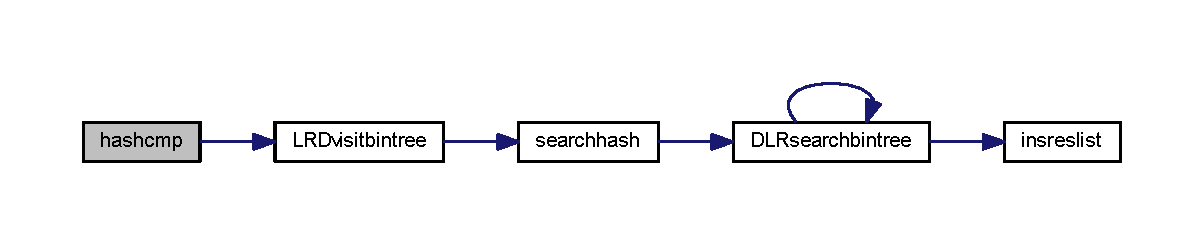
\includegraphics[width=350pt]{_function_8h_a5a318354c875367310f84de442acee2e_cgraph}
\end{center}
\end{figure}
这是这个函数的调用关系图\+:
\nopagebreak
\begin{figure}[H]
\begin{center}
\leavevmode
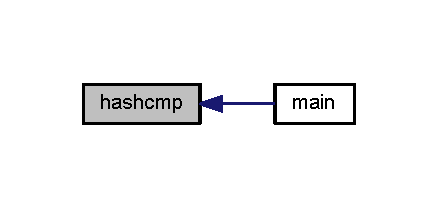
\includegraphics[width=210pt]{_function_8h_a5a318354c875367310f84de442acee2e_icgraph}
\end{center}
\end{figure}
\mbox{\Hypertarget{_function_8h_a1e3b6d38df0786ccf7f938d60e386aae}\label{_function_8h_a1e3b6d38df0786ccf7f938d60e386aae}} 
\index{Function.\+h@{Function.\+h}!Init@{Init}}
\index{Init@{Init}!Function.\+h@{Function.\+h}}
\subsubsection{\texorpdfstring{Init()}{Init()}}
{\footnotesize\ttfamily void Init (\begin{DoxyParamCaption}{ }\end{DoxyParamCaption})}



在文件 Init\+G\+U\+I.\+h 第 3 行定义.

这是这个函数的调用关系图\+:
\nopagebreak
\begin{figure}[H]
\begin{center}
\leavevmode
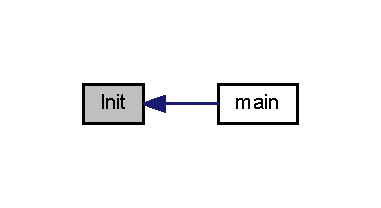
\includegraphics[width=183pt]{_function_8h_a1e3b6d38df0786ccf7f938d60e386aae_icgraph}
\end{center}
\end{figure}
\mbox{\Hypertarget{_function_8h_ae3057c044e96d31c1b28f1308551acbb}\label{_function_8h_ae3057c044e96d31c1b28f1308551acbb}} 
\index{Function.\+h@{Function.\+h}!insbintree@{insbintree}}
\index{insbintree@{insbintree}!Function.\+h@{Function.\+h}}
\subsubsection{\texorpdfstring{insbintree()}{insbintree()}}
{\footnotesize\ttfamily int insbintree (\begin{DoxyParamCaption}\item[{\hyperlink{_b_i_n_node_8h_a2fdaf7327a729b00aa89b6f5e3d6d336}{bin\+Tree\+N\+O\+DE} $\ast$}]{,  }\item[{\hyperlink{_b_i_n_node_8h_a2fdaf7327a729b00aa89b6f5e3d6d336}{bin\+Tree\+N\+O\+DE} $\ast$}]{ }\end{DoxyParamCaption})}



在文件 ins\+Bin\+Tree.\+h 第 6 行定义.

这是这个函数的调用关系图\+:
\nopagebreak
\begin{figure}[H]
\begin{center}
\leavevmode
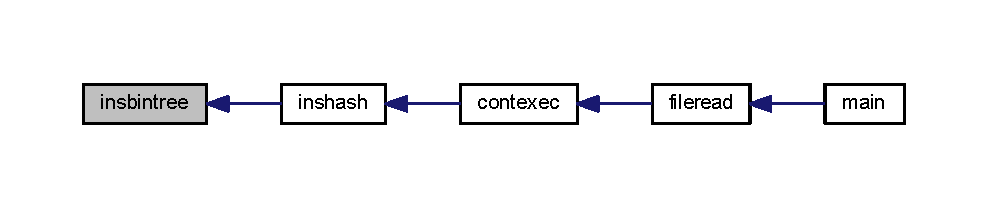
\includegraphics[width=350pt]{_function_8h_ae3057c044e96d31c1b28f1308551acbb_icgraph}
\end{center}
\end{figure}
\mbox{\Hypertarget{_function_8h_a7178f51f223e60c091b7c765abeba469}\label{_function_8h_a7178f51f223e60c091b7c765abeba469}} 
\index{Function.\+h@{Function.\+h}!inshash@{inshash}}
\index{inshash@{inshash}!Function.\+h@{Function.\+h}}
\subsubsection{\texorpdfstring{inshash()}{inshash()}}
{\footnotesize\ttfamily int inshash (\begin{DoxyParamCaption}\item[{\hyperlink{_b_i_n_node_8h_a2fdaf7327a729b00aa89b6f5e3d6d336}{bin\+Tree\+N\+O\+DE} $\ast$}]{hashT\mbox{[}$\,$\mbox{]},  }\item[{\hyperlink{_b_i_n_node_8h_a2fdaf7327a729b00aa89b6f5e3d6d336}{bin\+Tree\+N\+O\+DE} $\ast$}]{item }\end{DoxyParamCaption})}



在文件 ins\+Hash.\+h 第 12 行定义.

函数调用图\+:
\nopagebreak
\begin{figure}[H]
\begin{center}
\leavevmode
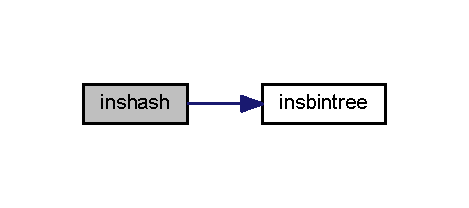
\includegraphics[width=225pt]{_function_8h_a7178f51f223e60c091b7c765abeba469_cgraph}
\end{center}
\end{figure}
这是这个函数的调用关系图\+:
\nopagebreak
\begin{figure}[H]
\begin{center}
\leavevmode
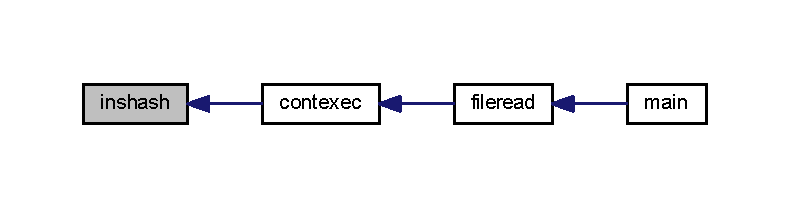
\includegraphics[width=350pt]{_function_8h_a7178f51f223e60c091b7c765abeba469_icgraph}
\end{center}
\end{figure}
\mbox{\Hypertarget{_function_8h_a1021ef2a4552ed9174ab6bd0f9e0b77a}\label{_function_8h_a1021ef2a4552ed9174ab6bd0f9e0b77a}} 
\index{Function.\+h@{Function.\+h}!insreslist@{insreslist}}
\index{insreslist@{insreslist}!Function.\+h@{Function.\+h}}
\subsubsection{\texorpdfstring{insreslist()}{insreslist()}}
{\footnotesize\ttfamily int insreslist (\begin{DoxyParamCaption}\item[{\hyperlink{res_node_8h_a99a496180780a83679ea667c9bc79fec}{res\+N\+O\+DE} $\ast$}]{list,  }\item[{\hyperlink{res_node_8h_a99a496180780a83679ea667c9bc79fec}{res\+N\+O\+DE} $\ast$}]{p }\end{DoxyParamCaption})}



在文件 Ins\+Res\+List.\+h 第 5 行定义.

这是这个函数的调用关系图\+:
\nopagebreak
\begin{figure}[H]
\begin{center}
\leavevmode
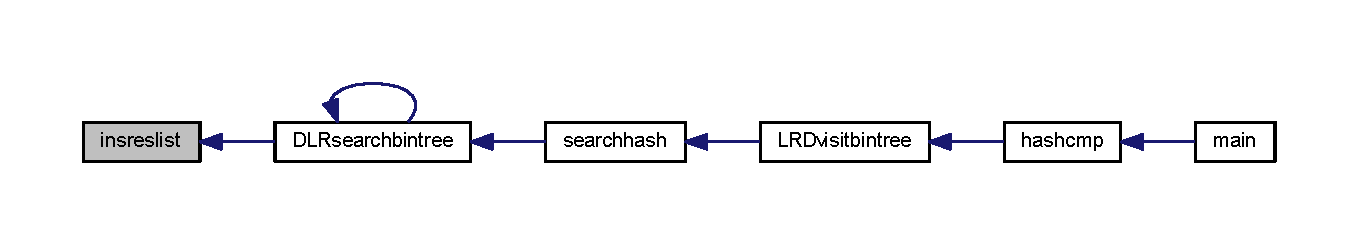
\includegraphics[width=350pt]{_function_8h_a1021ef2a4552ed9174ab6bd0f9e0b77a_icgraph}
\end{center}
\end{figure}
\mbox{\Hypertarget{_function_8h_af78bb1b244bd36a7f9007b7f9648fd6a}\label{_function_8h_af78bb1b244bd36a7f9007b7f9648fd6a}} 
\index{Function.\+h@{Function.\+h}!is\+Chinese@{is\+Chinese}}
\index{is\+Chinese@{is\+Chinese}!Function.\+h@{Function.\+h}}
\subsubsection{\texorpdfstring{is\+Chinese()}{isChinese()}}
{\footnotesize\ttfamily int is\+Chinese (\begin{DoxyParamCaption}\item[{char $\ast$}]{ }\end{DoxyParamCaption})}



在文件 is\+Chinese.\+h 第 4 行定义.

\mbox{\Hypertarget{_function_8h_ad40e7a9497ff7a575f32784f4887fc7c}\label{_function_8h_ad40e7a9497ff7a575f32784f4887fc7c}} 
\index{Function.\+h@{Function.\+h}!kmp@{kmp}}
\index{kmp@{kmp}!Function.\+h@{Function.\+h}}
\subsubsection{\texorpdfstring{kmp()}{kmp()}}
{\footnotesize\ttfamily long kmp (\begin{DoxyParamCaption}\item[{char $\ast$}]{master,  }\item[{char $\ast$}]{pattern,  }\item[{long}]{pos }\end{DoxyParamCaption})}



在文件 K\+M\+P.\+h 第 26 行定义.

函数调用图\+:
\nopagebreak
\begin{figure}[H]
\begin{center}
\leavevmode
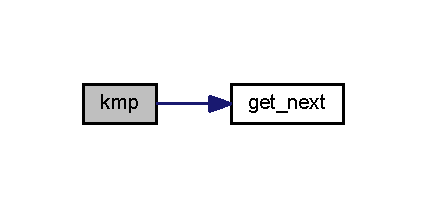
\includegraphics[width=205pt]{_function_8h_ad40e7a9497ff7a575f32784f4887fc7c_cgraph}
\end{center}
\end{figure}
这是这个函数的调用关系图\+:
\nopagebreak
\begin{figure}[H]
\begin{center}
\leavevmode
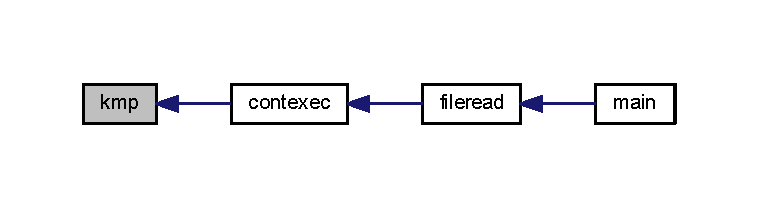
\includegraphics[width=350pt]{_function_8h_ad40e7a9497ff7a575f32784f4887fc7c_icgraph}
\end{center}
\end{figure}
\mbox{\Hypertarget{_function_8h_a98ae0a41ca54ee951b33e6561dd0572b}\label{_function_8h_a98ae0a41ca54ee951b33e6561dd0572b}} 
\index{Function.\+h@{Function.\+h}!L\+R\+D\+Clear\+Bin\+Tree@{L\+R\+D\+Clear\+Bin\+Tree}}
\index{L\+R\+D\+Clear\+Bin\+Tree@{L\+R\+D\+Clear\+Bin\+Tree}!Function.\+h@{Function.\+h}}
\subsubsection{\texorpdfstring{L\+R\+D\+Clear\+Bin\+Tree()}{LRDClearBinTree()}}
{\footnotesize\ttfamily int L\+R\+D\+Clear\+Bin\+Tree (\begin{DoxyParamCaption}\item[{\hyperlink{_b_i_n_node_8h_a2fdaf7327a729b00aa89b6f5e3d6d336}{bin\+Tree\+N\+O\+DE} $\ast$}]{bintree }\end{DoxyParamCaption})}



在文件 L\+R\+D\+Clear\+Bin\+Tree.\+h 第 5 行定义.

\mbox{\Hypertarget{_function_8h_a9164bd1b5c092f69060bdd4285f8917c}\label{_function_8h_a9164bd1b5c092f69060bdd4285f8917c}} 
\index{Function.\+h@{Function.\+h}!L\+R\+Dvisitbintree@{L\+R\+Dvisitbintree}}
\index{L\+R\+Dvisitbintree@{L\+R\+Dvisitbintree}!Function.\+h@{Function.\+h}}
\subsubsection{\texorpdfstring{L\+R\+Dvisitbintree()}{LRDvisitbintree()}}
{\footnotesize\ttfamily int L\+R\+Dvisitbintree (\begin{DoxyParamCaption}\item[{\hyperlink{_b_i_n_node_8h_a2fdaf7327a729b00aa89b6f5e3d6d336}{bin\+Tree\+N\+O\+DE} $\ast$}]{bintree,  }\item[{\hyperlink{_b_i_n_node_8h_a2fdaf7327a729b00aa89b6f5e3d6d336}{bin\+Tree\+N\+O\+DE} $\ast$}]{hashB\mbox{[}$\,$\mbox{]},  }\item[{\hyperlink{res_node_8h_a99a496180780a83679ea667c9bc79fec}{res\+N\+O\+DE} $\ast$}]{res\+List }\end{DoxyParamCaption})}



在文件 L\+R\+D\+Visit\+Bin\+Tree.\+h 第 3 行定义.

函数调用图\+:
\nopagebreak
\begin{figure}[H]
\begin{center}
\leavevmode
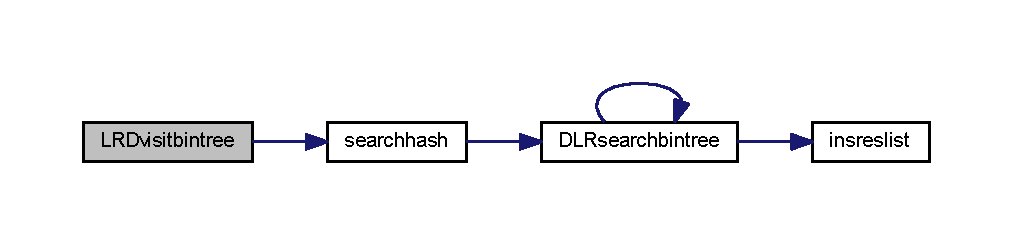
\includegraphics[width=350pt]{_function_8h_a9164bd1b5c092f69060bdd4285f8917c_cgraph}
\end{center}
\end{figure}
这是这个函数的调用关系图\+:
\nopagebreak
\begin{figure}[H]
\begin{center}
\leavevmode
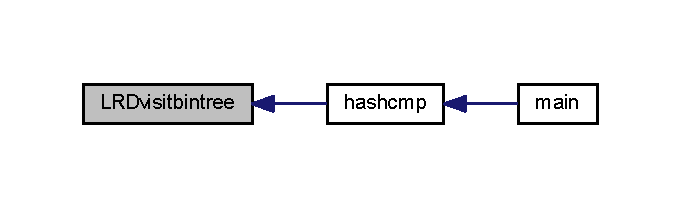
\includegraphics[width=327pt]{_function_8h_a9164bd1b5c092f69060bdd4285f8917c_icgraph}
\end{center}
\end{figure}
\mbox{\Hypertarget{_function_8h_a10b2b9a305b4ff344a5018171901a661}\label{_function_8h_a10b2b9a305b4ff344a5018171901a661}} 
\index{Function.\+h@{Function.\+h}!Pop\+Stack@{Pop\+Stack}}
\index{Pop\+Stack@{Pop\+Stack}!Function.\+h@{Function.\+h}}
\subsubsection{\texorpdfstring{Pop\+Stack()}{PopStack()}}
{\footnotesize\ttfamily \hyperlink{_s_t_a_c_k_n_o_d_e_8h_a29d53fde99d01064acfd82258fbc54d7}{S\+T\+A\+CK}$\ast$ Pop\+Stack (\begin{DoxyParamCaption}\item[{\hyperlink{_s_t_a_c_k_n_o_d_e_8h_a29d53fde99d01064acfd82258fbc54d7}{S\+T\+A\+CK} $\ast$}]{stack }\end{DoxyParamCaption})}



在文件 Pop\+Stack.\+h 第 3 行定义.

\mbox{\Hypertarget{_function_8h_a60c4ee271e18fa873ee5365cd50b8b53}\label{_function_8h_a60c4ee271e18fa873ee5365cd50b8b53}} 
\index{Function.\+h@{Function.\+h}!Push\+Stack@{Push\+Stack}}
\index{Push\+Stack@{Push\+Stack}!Function.\+h@{Function.\+h}}
\subsubsection{\texorpdfstring{Push\+Stack()}{PushStack()}}
{\footnotesize\ttfamily int Push\+Stack (\begin{DoxyParamCaption}\item[{\hyperlink{_s_t_a_c_k_n_o_d_e_8h_a29d53fde99d01064acfd82258fbc54d7}{S\+T\+A\+CK} $\ast$}]{stack,  }\item[{\hyperlink{_s_t_a_c_k_n_o_d_e_8h_a29d53fde99d01064acfd82258fbc54d7}{S\+T\+A\+CK} $\ast$}]{item }\end{DoxyParamCaption})}



在文件 Push\+Stack.\+h 第 3 行定义.

\mbox{\Hypertarget{_function_8h_acb0a1c9171ae96f2076bffd6dfe752e3}\label{_function_8h_acb0a1c9171ae96f2076bffd6dfe752e3}} 
\index{Function.\+h@{Function.\+h}!Quick\+Sort@{Quick\+Sort}}
\index{Quick\+Sort@{Quick\+Sort}!Function.\+h@{Function.\+h}}
\subsubsection{\texorpdfstring{Quick\+Sort()}{QuickSort()}}
{\footnotesize\ttfamily int Quick\+Sort (\begin{DoxyParamCaption}\item[{\hyperlink{res_node_8h_a99a496180780a83679ea667c9bc79fec}{res\+N\+O\+DE} $\ast$}]{list,  }\item[{\hyperlink{res_node_8h_a99a496180780a83679ea667c9bc79fec}{res\+N\+O\+DE} $\ast$}]{end }\end{DoxyParamCaption})}



在文件 Quick\+Sort.\+h 第 3 行定义.

这是这个函数的调用关系图\+:
\nopagebreak
\begin{figure}[H]
\begin{center}
\leavevmode
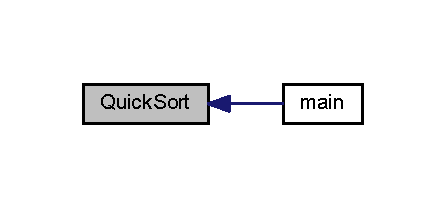
\includegraphics[width=214pt]{_function_8h_acb0a1c9171ae96f2076bffd6dfe752e3_icgraph}
\end{center}
\end{figure}
\mbox{\Hypertarget{_function_8h_a3cb1827c44099e76fe08fe6e409445fa}\label{_function_8h_a3cb1827c44099e76fe08fe6e409445fa}} 
\index{Function.\+h@{Function.\+h}!searchhash@{searchhash}}
\index{searchhash@{searchhash}!Function.\+h@{Function.\+h}}
\subsubsection{\texorpdfstring{searchhash()}{searchhash()}}
{\footnotesize\ttfamily int searchhash (\begin{DoxyParamCaption}\item[{\hyperlink{_b_i_n_node_8h_a2fdaf7327a729b00aa89b6f5e3d6d336}{bin\+Tree\+N\+O\+DE} $\ast$}]{bintree,  }\item[{\hyperlink{_b_i_n_node_8h_a2fdaf7327a729b00aa89b6f5e3d6d336}{bin\+Tree\+N\+O\+DE} $\ast$}]{hashB\mbox{[}$\,$\mbox{]},  }\item[{\hyperlink{res_node_8h_a99a496180780a83679ea667c9bc79fec}{res\+N\+O\+DE} $\ast$}]{res\+List }\end{DoxyParamCaption})}



在文件 Search\+Hash.\+h 第 5 行定义.

函数调用图\+:
\nopagebreak
\begin{figure}[H]
\begin{center}
\leavevmode
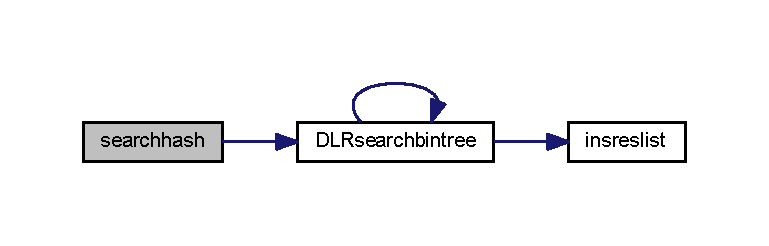
\includegraphics[width=350pt]{_function_8h_a3cb1827c44099e76fe08fe6e409445fa_cgraph}
\end{center}
\end{figure}
这是这个函数的调用关系图\+:
\nopagebreak
\begin{figure}[H]
\begin{center}
\leavevmode
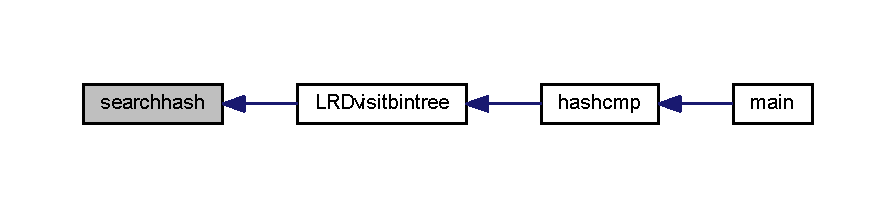
\includegraphics[width=350pt]{_function_8h_a3cb1827c44099e76fe08fe6e409445fa_icgraph}
\end{center}
\end{figure}
\mbox{\Hypertarget{_function_8h_a916d9eda097fba327f23e85b1af09821}\label{_function_8h_a916d9eda097fba327f23e85b1af09821}} 
\index{Function.\+h@{Function.\+h}!Show\+Result@{Show\+Result}}
\index{Show\+Result@{Show\+Result}!Function.\+h@{Function.\+h}}
\subsubsection{\texorpdfstring{Show\+Result()}{ShowResult()}}
{\footnotesize\ttfamily void Show\+Result (\begin{DoxyParamCaption}\item[{\hyperlink{res_node_8h_a99a496180780a83679ea667c9bc79fec}{res\+N\+O\+DE} $\ast$}]{list }\end{DoxyParamCaption})}



在文件 Show\+Result.\+h 第 3 行定义.

这是这个函数的调用关系图\+:
\nopagebreak
\begin{figure}[H]
\begin{center}
\leavevmode
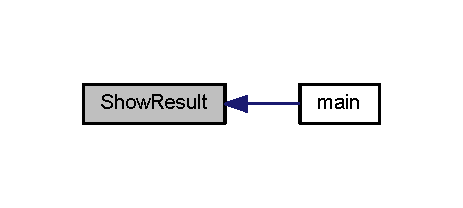
\includegraphics[width=222pt]{_function_8h_a916d9eda097fba327f23e85b1af09821_icgraph}
\end{center}
\end{figure}

\hypertarget{_hash_cmp_8h}{}\section{Hash\+Cmp.\+h 文件参考}
\label{_hash_cmp_8h}\index{Hash\+Cmp.\+h@{Hash\+Cmp.\+h}}
此图展示该文件直接或间接的被哪些文件引用了\+:
\nopagebreak
\begin{figure}[H]
\begin{center}
\leavevmode
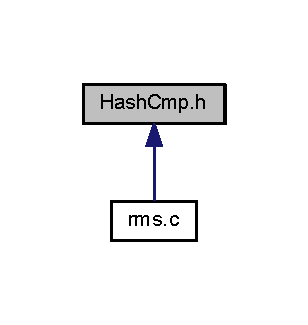
\includegraphics[width=148pt]{_hash_cmp_8h__dep__incl}
\end{center}
\end{figure}
\subsection*{函数}
\begin{DoxyCompactItemize}
\item 
int \hyperlink{_hash_cmp_8h_a5a318354c875367310f84de442acee2e}{hashcmp} (\hyperlink{_b_i_n_node_8h_a2fdaf7327a729b00aa89b6f5e3d6d336}{bin\+Tree\+N\+O\+DE} $\ast$hashA\mbox{[}$\,$\mbox{]}, \hyperlink{_b_i_n_node_8h_a2fdaf7327a729b00aa89b6f5e3d6d336}{bin\+Tree\+N\+O\+DE} $\ast$hashB\mbox{[}$\,$\mbox{]}, \hyperlink{res_node_8h_a99a496180780a83679ea667c9bc79fec}{res\+N\+O\+DE} $\ast$res\+List)
\end{DoxyCompactItemize}


\subsection{函数说明}
\mbox{\Hypertarget{_hash_cmp_8h_a5a318354c875367310f84de442acee2e}\label{_hash_cmp_8h_a5a318354c875367310f84de442acee2e}} 
\index{Hash\+Cmp.\+h@{Hash\+Cmp.\+h}!hashcmp@{hashcmp}}
\index{hashcmp@{hashcmp}!Hash\+Cmp.\+h@{Hash\+Cmp.\+h}}
\subsubsection{\texorpdfstring{hashcmp()}{hashcmp()}}
{\footnotesize\ttfamily int hashcmp (\begin{DoxyParamCaption}\item[{\hyperlink{_b_i_n_node_8h_a2fdaf7327a729b00aa89b6f5e3d6d336}{bin\+Tree\+N\+O\+DE} $\ast$}]{hashA\mbox{[}$\,$\mbox{]},  }\item[{\hyperlink{_b_i_n_node_8h_a2fdaf7327a729b00aa89b6f5e3d6d336}{bin\+Tree\+N\+O\+DE} $\ast$}]{hashB\mbox{[}$\,$\mbox{]},  }\item[{\hyperlink{res_node_8h_a99a496180780a83679ea667c9bc79fec}{res\+N\+O\+DE} $\ast$}]{res\+List }\end{DoxyParamCaption})}



在文件 Hash\+Cmp.\+h 第 5 行定义.

函数调用图\+:
\nopagebreak
\begin{figure}[H]
\begin{center}
\leavevmode
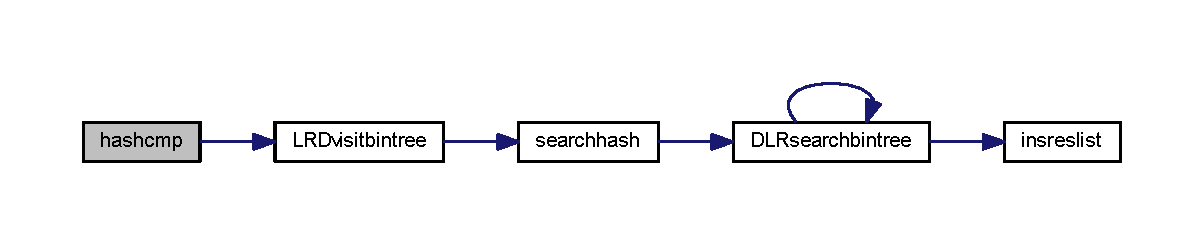
\includegraphics[width=350pt]{_hash_cmp_8h_a5a318354c875367310f84de442acee2e_cgraph}
\end{center}
\end{figure}
这是这个函数的调用关系图\+:
\nopagebreak
\begin{figure}[H]
\begin{center}
\leavevmode
\includegraphics[width=210pt]{_hash_cmp_8h_a5a318354c875367310f84de442acee2e_icgraph}
\end{center}
\end{figure}

\hypertarget{_init_g_u_i_8h}{}\section{Init\+G\+U\+I.\+h 文件参考}
\label{_init_g_u_i_8h}\index{Init\+G\+U\+I.\+h@{Init\+G\+U\+I.\+h}}
此图展示该文件直接或间接的被哪些文件引用了\+:
\nopagebreak
\begin{figure}[H]
\begin{center}
\leavevmode
\includegraphics[width=134pt]{_init_g_u_i_8h__dep__incl}
\end{center}
\end{figure}
\subsection*{函数}
\begin{DoxyCompactItemize}
\item 
void \hyperlink{_init_g_u_i_8h_a1e3b6d38df0786ccf7f938d60e386aae}{Init} ()
\end{DoxyCompactItemize}


\subsection{函数说明}
\mbox{\Hypertarget{_init_g_u_i_8h_a1e3b6d38df0786ccf7f938d60e386aae}\label{_init_g_u_i_8h_a1e3b6d38df0786ccf7f938d60e386aae}} 
\index{Init\+G\+U\+I.\+h@{Init\+G\+U\+I.\+h}!Init@{Init}}
\index{Init@{Init}!Init\+G\+U\+I.\+h@{Init\+G\+U\+I.\+h}}
\subsubsection{\texorpdfstring{Init()}{Init()}}
{\footnotesize\ttfamily void Init (\begin{DoxyParamCaption}{ }\end{DoxyParamCaption})}



在文件 Init\+G\+U\+I.\+h 第 3 行定义.

这是这个函数的调用关系图\+:
\nopagebreak
\begin{figure}[H]
\begin{center}
\leavevmode
\includegraphics[width=183pt]{_init_g_u_i_8h_a1e3b6d38df0786ccf7f938d60e386aae_icgraph}
\end{center}
\end{figure}

\hypertarget{ins_bin_tree_8h}{}\section{ins\+Bin\+Tree.\+h 文件参考}
\label{ins_bin_tree_8h}\index{ins\+Bin\+Tree.\+h@{ins\+Bin\+Tree.\+h}}
{\ttfamily \#include $<$string.\+h$>$}\newline
ins\+Bin\+Tree.\+h 的引用(Include)关系图\+:
\nopagebreak
\begin{figure}[H]
\begin{center}
\leavevmode
\includegraphics[width=151pt]{ins_bin_tree_8h__incl}
\end{center}
\end{figure}
此图展示该文件直接或间接的被哪些文件引用了\+:
\nopagebreak
\begin{figure}[H]
\begin{center}
\leavevmode
\includegraphics[width=175pt]{ins_bin_tree_8h__dep__incl}
\end{center}
\end{figure}
\subsection*{函数}
\begin{DoxyCompactItemize}
\item 
int \hyperlink{ins_bin_tree_8h_a6d7fb2bcc5a546988d63d0f56e39b7ed}{insbintree} (struct \hyperlink{struct_b_i_n_t_r_e_e}{B\+I\+N\+T\+R\+EE} $\ast$bintree, struct \hyperlink{struct_b_i_n_t_r_e_e}{B\+I\+N\+T\+R\+EE} $\ast$item)
\end{DoxyCompactItemize}


\subsection{函数说明}
\mbox{\Hypertarget{ins_bin_tree_8h_a6d7fb2bcc5a546988d63d0f56e39b7ed}\label{ins_bin_tree_8h_a6d7fb2bcc5a546988d63d0f56e39b7ed}} 
\index{ins\+Bin\+Tree.\+h@{ins\+Bin\+Tree.\+h}!insbintree@{insbintree}}
\index{insbintree@{insbintree}!ins\+Bin\+Tree.\+h@{ins\+Bin\+Tree.\+h}}
\subsubsection{\texorpdfstring{insbintree()}{insbintree()}}
{\footnotesize\ttfamily int insbintree (\begin{DoxyParamCaption}\item[{struct \hyperlink{struct_b_i_n_t_r_e_e}{B\+I\+N\+T\+R\+EE} $\ast$}]{bintree,  }\item[{struct \hyperlink{struct_b_i_n_t_r_e_e}{B\+I\+N\+T\+R\+EE} $\ast$}]{item }\end{DoxyParamCaption})}



在文件 ins\+Bin\+Tree.\+h 第 6 行定义.

这是这个函数的调用关系图\+:
\nopagebreak
\begin{figure}[H]
\begin{center}
\leavevmode
\includegraphics[width=350pt]{ins_bin_tree_8h_a6d7fb2bcc5a546988d63d0f56e39b7ed_icgraph}
\end{center}
\end{figure}

\hypertarget{ins_hash_8h}{}\section{ins\+Hash.\+h 文件参考}
\label{ins_hash_8h}\index{ins\+Hash.\+h@{ins\+Hash.\+h}}
{\ttfamily \#include $<$string.\+h$>$}\newline
{\ttfamily \#include $<$stdlib.\+h$>$}\newline
{\ttfamily \#include $<$stdio.\+h$>$}\newline
{\ttfamily \#include \char`\"{}B\+I\+N\+Node.\+h\char`\"{}}\newline
{\ttfamily \#include \char`\"{}Member\+Node.\+h\char`\"{}}\newline
{\ttfamily \#include \char`\"{}ins\+Bin\+Tree.\+h\char`\"{}}\newline
ins\+Hash.\+h 的引用(Include)关系图\+:
\nopagebreak
\begin{figure}[H]
\begin{center}
\leavevmode
\includegraphics[width=350pt]{ins_hash_8h__incl}
\end{center}
\end{figure}
此图展示该文件直接或间接的被哪些文件引用了\+:
\nopagebreak
\begin{figure}[H]
\begin{center}
\leavevmode
\includegraphics[width=140pt]{ins_hash_8h__dep__incl}
\end{center}
\end{figure}
\subsection*{函数}
\begin{DoxyCompactItemize}
\item 
int \hyperlink{ins_hash_8h_a7178f51f223e60c091b7c765abeba469}{inshash} (\hyperlink{_b_i_n_node_8h_a2fdaf7327a729b00aa89b6f5e3d6d336}{bin\+Tree\+N\+O\+DE} $\ast$hashT\mbox{[}$\,$\mbox{]}, \hyperlink{_b_i_n_node_8h_a2fdaf7327a729b00aa89b6f5e3d6d336}{bin\+Tree\+N\+O\+DE} $\ast$item)
\end{DoxyCompactItemize}


\subsection{函数说明}
\mbox{\Hypertarget{ins_hash_8h_a7178f51f223e60c091b7c765abeba469}\label{ins_hash_8h_a7178f51f223e60c091b7c765abeba469}} 
\index{ins\+Hash.\+h@{ins\+Hash.\+h}!inshash@{inshash}}
\index{inshash@{inshash}!ins\+Hash.\+h@{ins\+Hash.\+h}}
\subsubsection{\texorpdfstring{inshash()}{inshash()}}
{\footnotesize\ttfamily int inshash (\begin{DoxyParamCaption}\item[{\hyperlink{_b_i_n_node_8h_a2fdaf7327a729b00aa89b6f5e3d6d336}{bin\+Tree\+N\+O\+DE} $\ast$}]{hashT\mbox{[}$\,$\mbox{]},  }\item[{\hyperlink{_b_i_n_node_8h_a2fdaf7327a729b00aa89b6f5e3d6d336}{bin\+Tree\+N\+O\+DE} $\ast$}]{item }\end{DoxyParamCaption})}



在文件 ins\+Hash.\+h 第 12 行定义.

函数调用图\+:
\nopagebreak
\begin{figure}[H]
\begin{center}
\leavevmode
\includegraphics[width=225pt]{ins_hash_8h_a7178f51f223e60c091b7c765abeba469_cgraph}
\end{center}
\end{figure}
这是这个函数的调用关系图\+:
\nopagebreak
\begin{figure}[H]
\begin{center}
\leavevmode
\includegraphics[width=350pt]{ins_hash_8h_a7178f51f223e60c091b7c765abeba469_icgraph}
\end{center}
\end{figure}

\hypertarget{_ins_res_list_8h}{}\section{Ins\+Res\+List.\+h 文件参考}
\label{_ins_res_list_8h}\index{Ins\+Res\+List.\+h@{Ins\+Res\+List.\+h}}
{\ttfamily \#include \char`\"{}res\+Node.\+h\char`\"{}}\newline
Ins\+Res\+List.\+h 的引用(Include)关系图\+:
\nopagebreak
\begin{figure}[H]
\begin{center}
\leavevmode
\includegraphics[width=151pt]{_ins_res_list_8h__incl}
\end{center}
\end{figure}
此图展示该文件直接或间接的被哪些文件引用了\+:
\nopagebreak
\begin{figure}[H]
\begin{center}
\leavevmode
\includegraphics[width=151pt]{_ins_res_list_8h__dep__incl}
\end{center}
\end{figure}
\subsection*{函数}
\begin{DoxyCompactItemize}
\item 
int \hyperlink{_ins_res_list_8h_a1021ef2a4552ed9174ab6bd0f9e0b77a}{insreslist} (\hyperlink{res_node_8h_a99a496180780a83679ea667c9bc79fec}{res\+N\+O\+DE} $\ast$list, \hyperlink{res_node_8h_a99a496180780a83679ea667c9bc79fec}{res\+N\+O\+DE} $\ast$p)
\end{DoxyCompactItemize}


\subsection{函数说明}
\mbox{\Hypertarget{_ins_res_list_8h_a1021ef2a4552ed9174ab6bd0f9e0b77a}\label{_ins_res_list_8h_a1021ef2a4552ed9174ab6bd0f9e0b77a}} 
\index{Ins\+Res\+List.\+h@{Ins\+Res\+List.\+h}!insreslist@{insreslist}}
\index{insreslist@{insreslist}!Ins\+Res\+List.\+h@{Ins\+Res\+List.\+h}}
\subsubsection{\texorpdfstring{insreslist()}{insreslist()}}
{\footnotesize\ttfamily int insreslist (\begin{DoxyParamCaption}\item[{\hyperlink{res_node_8h_a99a496180780a83679ea667c9bc79fec}{res\+N\+O\+DE} $\ast$}]{list,  }\item[{\hyperlink{res_node_8h_a99a496180780a83679ea667c9bc79fec}{res\+N\+O\+DE} $\ast$}]{p }\end{DoxyParamCaption})}



在文件 Ins\+Res\+List.\+h 第 5 行定义.

这是这个函数的调用关系图\+:
\nopagebreak
\begin{figure}[H]
\begin{center}
\leavevmode
\includegraphics[width=350pt]{_ins_res_list_8h_a1021ef2a4552ed9174ab6bd0f9e0b77a_icgraph}
\end{center}
\end{figure}

\hypertarget{is_chinese_8h}{}\section{is\+Chinese.\+h 文件参考}
\label{is_chinese_8h}\index{is\+Chinese.\+h@{is\+Chinese.\+h}}
此图展示该文件直接或间接的被哪些文件引用了\+:
\nopagebreak
\begin{figure}[H]
\begin{center}
\leavevmode
\includegraphics[width=148pt]{is_chinese_8h__dep__incl}
\end{center}
\end{figure}
\subsection*{函数}
\begin{DoxyCompactItemize}
\item 
int \hyperlink{is_chinese_8h_a6c224aa3059c7b5cd8fd3bf7a5a2cab2}{is\+Chinese} (char $\ast$str)
\end{DoxyCompactItemize}


\subsection{函数说明}
\mbox{\Hypertarget{is_chinese_8h_a6c224aa3059c7b5cd8fd3bf7a5a2cab2}\label{is_chinese_8h_a6c224aa3059c7b5cd8fd3bf7a5a2cab2}} 
\index{is\+Chinese.\+h@{is\+Chinese.\+h}!is\+Chinese@{is\+Chinese}}
\index{is\+Chinese@{is\+Chinese}!is\+Chinese.\+h@{is\+Chinese.\+h}}
\subsubsection{\texorpdfstring{is\+Chinese()}{isChinese()}}
{\footnotesize\ttfamily int is\+Chinese (\begin{DoxyParamCaption}\item[{char $\ast$}]{str }\end{DoxyParamCaption})}



在文件 is\+Chinese.\+h 第 4 行定义.


\hypertarget{is_empty_stack_8h}{}\section{is\+Empty\+Stack.\+h 文件参考}
\label{is_empty_stack_8h}\index{is\+Empty\+Stack.\+h@{is\+Empty\+Stack.\+h}}
此图展示该文件直接或间接的被哪些文件引用了\+:
\nopagebreak
\begin{figure}[H]
\begin{center}
\leavevmode
\includegraphics[width=166pt]{is_empty_stack_8h__dep__incl}
\end{center}
\end{figure}
\subsection*{函数}
\begin{DoxyCompactItemize}
\item 
int \hyperlink{is_empty_stack_8h_ab5ed91b2bc4c60c05d32224286d195d7}{is\+Empty\+Stack} (struct \hyperlink{struct_s_t_a_c_k_n_o_d_e}{S\+T\+A\+C\+K\+N\+O\+DE} $\ast$stack)
\end{DoxyCompactItemize}


\subsection{函数说明}
\mbox{\Hypertarget{is_empty_stack_8h_ab5ed91b2bc4c60c05d32224286d195d7}\label{is_empty_stack_8h_ab5ed91b2bc4c60c05d32224286d195d7}} 
\index{is\+Empty\+Stack.\+h@{is\+Empty\+Stack.\+h}!is\+Empty\+Stack@{is\+Empty\+Stack}}
\index{is\+Empty\+Stack@{is\+Empty\+Stack}!is\+Empty\+Stack.\+h@{is\+Empty\+Stack.\+h}}
\subsubsection{\texorpdfstring{is\+Empty\+Stack()}{isEmptyStack()}}
{\footnotesize\ttfamily int is\+Empty\+Stack (\begin{DoxyParamCaption}\item[{struct \hyperlink{struct_s_t_a_c_k_n_o_d_e}{S\+T\+A\+C\+K\+N\+O\+DE} $\ast$}]{stack }\end{DoxyParamCaption})}



在文件 is\+Empty\+Stack.\+h 第 3 行定义.


\hypertarget{_k_m_p_8h}{}\section{K\+M\+P.\+h 文件参考}
\label{_k_m_p_8h}\index{K\+M\+P.\+h@{K\+M\+P.\+h}}
{\ttfamily \#include $<$malloc.\+h$>$}\newline
K\+M\+P.\+h 的引用(Include)关系图\+:
\nopagebreak
\begin{figure}[H]
\begin{center}
\leavevmode
\includegraphics[width=133pt]{_k_m_p_8h__incl}
\end{center}
\end{figure}
此图展示该文件直接或间接的被哪些文件引用了\+:
\nopagebreak
\begin{figure}[H]
\begin{center}
\leavevmode
\includegraphics[width=127pt]{_k_m_p_8h__dep__incl}
\end{center}
\end{figure}
\subsection*{函数}
\begin{DoxyCompactItemize}
\item 
void \hyperlink{_k_m_p_8h_ab654cff237f25550252e4eb40971c8f5}{get\+\_\+next} (char $\ast$str, int next\mbox{[}$\,$\mbox{]}, int str\+Length)
\item 
long \hyperlink{_k_m_p_8h_ad40e7a9497ff7a575f32784f4887fc7c}{kmp} (char $\ast$master, char $\ast$pattern, long pos)
\end{DoxyCompactItemize}


\subsection{函数说明}
\mbox{\Hypertarget{_k_m_p_8h_ab654cff237f25550252e4eb40971c8f5}\label{_k_m_p_8h_ab654cff237f25550252e4eb40971c8f5}} 
\index{K\+M\+P.\+h@{K\+M\+P.\+h}!get\+\_\+next@{get\+\_\+next}}
\index{get\+\_\+next@{get\+\_\+next}!K\+M\+P.\+h@{K\+M\+P.\+h}}
\subsubsection{\texorpdfstring{get\+\_\+next()}{get\_next()}}
{\footnotesize\ttfamily void get\+\_\+next (\begin{DoxyParamCaption}\item[{char $\ast$}]{str,  }\item[{int}]{next\mbox{[}$\,$\mbox{]},  }\item[{int}]{str\+Length }\end{DoxyParamCaption})}



在文件 K\+M\+P.\+h 第 4 行定义.

这是这个函数的调用关系图\+:
\nopagebreak
\begin{figure}[H]
\begin{center}
\leavevmode
\includegraphics[width=350pt]{_k_m_p_8h_ab654cff237f25550252e4eb40971c8f5_icgraph}
\end{center}
\end{figure}
\mbox{\Hypertarget{_k_m_p_8h_ad40e7a9497ff7a575f32784f4887fc7c}\label{_k_m_p_8h_ad40e7a9497ff7a575f32784f4887fc7c}} 
\index{K\+M\+P.\+h@{K\+M\+P.\+h}!kmp@{kmp}}
\index{kmp@{kmp}!K\+M\+P.\+h@{K\+M\+P.\+h}}
\subsubsection{\texorpdfstring{kmp()}{kmp()}}
{\footnotesize\ttfamily long kmp (\begin{DoxyParamCaption}\item[{char $\ast$}]{master,  }\item[{char $\ast$}]{pattern,  }\item[{long}]{pos }\end{DoxyParamCaption})}



在文件 K\+M\+P.\+h 第 26 行定义.

函数调用图\+:
\nopagebreak
\begin{figure}[H]
\begin{center}
\leavevmode
\includegraphics[width=205pt]{_k_m_p_8h_ad40e7a9497ff7a575f32784f4887fc7c_cgraph}
\end{center}
\end{figure}
这是这个函数的调用关系图\+:
\nopagebreak
\begin{figure}[H]
\begin{center}
\leavevmode
\includegraphics[width=350pt]{_k_m_p_8h_ad40e7a9497ff7a575f32784f4887fc7c_icgraph}
\end{center}
\end{figure}

\hypertarget{_l_r_d_clear_bin_tree_8h}{}\section{L\+R\+D\+Clear\+Bin\+Tree.\+h 文件参考}
\label{_l_r_d_clear_bin_tree_8h}\index{L\+R\+D\+Clear\+Bin\+Tree.\+h@{L\+R\+D\+Clear\+Bin\+Tree.\+h}}
{\ttfamily \#include $<$malloc.\+h$>$}\newline
{\ttfamily \#include \char`\"{}B\+I\+N\+Node.\+h\char`\"{}}\newline
L\+R\+D\+Clear\+Bin\+Tree.\+h 的引用(Include)关系图\+:
\nopagebreak
\begin{figure}[H]
\begin{center}
\leavevmode
\includegraphics[width=214pt]{_l_r_d_clear_bin_tree_8h__incl}
\end{center}
\end{figure}
此图展示该文件直接或间接的被哪些文件引用了\+:
\nopagebreak
\begin{figure}[H]
\begin{center}
\leavevmode
\includegraphics[width=179pt]{_l_r_d_clear_bin_tree_8h__dep__incl}
\end{center}
\end{figure}
\subsection*{函数}
\begin{DoxyCompactItemize}
\item 
int \hyperlink{_l_r_d_clear_bin_tree_8h_a98ae0a41ca54ee951b33e6561dd0572b}{L\+R\+D\+Clear\+Bin\+Tree} (\hyperlink{_b_i_n_node_8h_a2fdaf7327a729b00aa89b6f5e3d6d336}{bin\+Tree\+N\+O\+DE} $\ast$bintree)
\end{DoxyCompactItemize}


\subsection{函数说明}
\mbox{\Hypertarget{_l_r_d_clear_bin_tree_8h_a98ae0a41ca54ee951b33e6561dd0572b}\label{_l_r_d_clear_bin_tree_8h_a98ae0a41ca54ee951b33e6561dd0572b}} 
\index{L\+R\+D\+Clear\+Bin\+Tree.\+h@{L\+R\+D\+Clear\+Bin\+Tree.\+h}!L\+R\+D\+Clear\+Bin\+Tree@{L\+R\+D\+Clear\+Bin\+Tree}}
\index{L\+R\+D\+Clear\+Bin\+Tree@{L\+R\+D\+Clear\+Bin\+Tree}!L\+R\+D\+Clear\+Bin\+Tree.\+h@{L\+R\+D\+Clear\+Bin\+Tree.\+h}}
\subsubsection{\texorpdfstring{L\+R\+D\+Clear\+Bin\+Tree()}{LRDClearBinTree()}}
{\footnotesize\ttfamily int L\+R\+D\+Clear\+Bin\+Tree (\begin{DoxyParamCaption}\item[{\hyperlink{_b_i_n_node_8h_a2fdaf7327a729b00aa89b6f5e3d6d336}{bin\+Tree\+N\+O\+DE} $\ast$}]{bintree }\end{DoxyParamCaption})}



在文件 L\+R\+D\+Clear\+Bin\+Tree.\+h 第 5 行定义.


\hypertarget{_l_r_d_visit_bin_tree_8h}{}\section{L\+R\+D\+Visit\+Bin\+Tree.\+h 文件参考}
\label{_l_r_d_visit_bin_tree_8h}\index{L\+R\+D\+Visit\+Bin\+Tree.\+h@{L\+R\+D\+Visit\+Bin\+Tree.\+h}}
此图展示该文件直接或间接的被哪些文件引用了\+:
\nopagebreak
\begin{figure}[H]
\begin{center}
\leavevmode
\includegraphics[width=176pt]{_l_r_d_visit_bin_tree_8h__dep__incl}
\end{center}
\end{figure}
\subsection*{函数}
\begin{DoxyCompactItemize}
\item 
int \hyperlink{_l_r_d_visit_bin_tree_8h_a9164bd1b5c092f69060bdd4285f8917c}{L\+R\+Dvisitbintree} (\hyperlink{_b_i_n_node_8h_a2fdaf7327a729b00aa89b6f5e3d6d336}{bin\+Tree\+N\+O\+DE} $\ast$bintree, \hyperlink{_b_i_n_node_8h_a2fdaf7327a729b00aa89b6f5e3d6d336}{bin\+Tree\+N\+O\+DE} $\ast$hashB\mbox{[}$\,$\mbox{]}, \hyperlink{res_node_8h_a99a496180780a83679ea667c9bc79fec}{res\+N\+O\+DE} $\ast$res\+List)
\end{DoxyCompactItemize}


\subsection{函数说明}
\mbox{\Hypertarget{_l_r_d_visit_bin_tree_8h_a9164bd1b5c092f69060bdd4285f8917c}\label{_l_r_d_visit_bin_tree_8h_a9164bd1b5c092f69060bdd4285f8917c}} 
\index{L\+R\+D\+Visit\+Bin\+Tree.\+h@{L\+R\+D\+Visit\+Bin\+Tree.\+h}!L\+R\+Dvisitbintree@{L\+R\+Dvisitbintree}}
\index{L\+R\+Dvisitbintree@{L\+R\+Dvisitbintree}!L\+R\+D\+Visit\+Bin\+Tree.\+h@{L\+R\+D\+Visit\+Bin\+Tree.\+h}}
\subsubsection{\texorpdfstring{L\+R\+Dvisitbintree()}{LRDvisitbintree()}}
{\footnotesize\ttfamily int L\+R\+Dvisitbintree (\begin{DoxyParamCaption}\item[{\hyperlink{_b_i_n_node_8h_a2fdaf7327a729b00aa89b6f5e3d6d336}{bin\+Tree\+N\+O\+DE} $\ast$}]{bintree,  }\item[{\hyperlink{_b_i_n_node_8h_a2fdaf7327a729b00aa89b6f5e3d6d336}{bin\+Tree\+N\+O\+DE} $\ast$}]{hashB\mbox{[}$\,$\mbox{]},  }\item[{\hyperlink{res_node_8h_a99a496180780a83679ea667c9bc79fec}{res\+N\+O\+DE} $\ast$}]{res\+List }\end{DoxyParamCaption})}



在文件 L\+R\+D\+Visit\+Bin\+Tree.\+h 第 3 行定义.

函数调用图\+:
\nopagebreak
\begin{figure}[H]
\begin{center}
\leavevmode
\includegraphics[width=350pt]{_l_r_d_visit_bin_tree_8h_a9164bd1b5c092f69060bdd4285f8917c_cgraph}
\end{center}
\end{figure}
这是这个函数的调用关系图\+:
\nopagebreak
\begin{figure}[H]
\begin{center}
\leavevmode
\includegraphics[width=327pt]{_l_r_d_visit_bin_tree_8h_a9164bd1b5c092f69060bdd4285f8917c_icgraph}
\end{center}
\end{figure}

\hypertarget{_member_node_8h}{}\section{Member\+Node.\+h 文件参考}
\label{_member_node_8h}\index{Member\+Node.\+h@{Member\+Node.\+h}}
此图展示该文件直接或间接的被哪些文件引用了\+:
\nopagebreak
\begin{figure}[H]
\begin{center}
\leavevmode
\includegraphics[width=298pt]{_member_node_8h__dep__incl}
\end{center}
\end{figure}
\subsection*{类}
\begin{DoxyCompactItemize}
\item 
struct \hyperlink{struct_m_e_m_b_e_r_n_o_d_e}{M\+E\+M\+B\+E\+R\+N\+O\+DE}
\end{DoxyCompactItemize}
\subsection*{类型定义}
\begin{DoxyCompactItemize}
\item 
typedef struct \hyperlink{struct_m_e_m_b_e_r_n_o_d_e}{M\+E\+M\+B\+E\+R\+N\+O\+DE} \hyperlink{_member_node_8h_af952c400512f5ff05a9356b68cb15730}{M\+N\+O\+DE}
\end{DoxyCompactItemize}


\subsection{类型定义说明}
\mbox{\Hypertarget{_member_node_8h_af952c400512f5ff05a9356b68cb15730}\label{_member_node_8h_af952c400512f5ff05a9356b68cb15730}} 
\index{Member\+Node.\+h@{Member\+Node.\+h}!M\+N\+O\+DE@{M\+N\+O\+DE}}
\index{M\+N\+O\+DE@{M\+N\+O\+DE}!Member\+Node.\+h@{Member\+Node.\+h}}
\subsubsection{\texorpdfstring{M\+N\+O\+DE}{MNODE}}
{\footnotesize\ttfamily typedef struct \hyperlink{struct_m_e_m_b_e_r_n_o_d_e}{M\+E\+M\+B\+E\+R\+N\+O\+DE} \hyperlink{_member_node_8h_af952c400512f5ff05a9356b68cb15730}{M\+N\+O\+DE}}


\hypertarget{_pop_stack_8h}{}\section{Pop\+Stack.\+h 文件参考}
\label{_pop_stack_8h}\index{Pop\+Stack.\+h@{Pop\+Stack.\+h}}
此图展示该文件直接或间接的被哪些文件引用了\+:
\nopagebreak
\begin{figure}[H]
\begin{center}
\leavevmode
\includegraphics[width=148pt]{_pop_stack_8h__dep__incl}
\end{center}
\end{figure}
\subsection*{函数}
\begin{DoxyCompactItemize}
\item 
struct \hyperlink{struct_s_t_a_c_k_n_o_d_e}{S\+T\+A\+C\+K\+N\+O\+DE} $\ast$ \hyperlink{_pop_stack_8h_a450fe136ec20038dedf161062d744b3b}{Pop\+Stack} (\hyperlink{_s_t_a_c_k_n_o_d_e_8h_a29d53fde99d01064acfd82258fbc54d7}{S\+T\+A\+CK} $\ast$stack)
\end{DoxyCompactItemize}


\subsection{函数说明}
\mbox{\Hypertarget{_pop_stack_8h_a450fe136ec20038dedf161062d744b3b}\label{_pop_stack_8h_a450fe136ec20038dedf161062d744b3b}} 
\index{Pop\+Stack.\+h@{Pop\+Stack.\+h}!Pop\+Stack@{Pop\+Stack}}
\index{Pop\+Stack@{Pop\+Stack}!Pop\+Stack.\+h@{Pop\+Stack.\+h}}
\subsubsection{\texorpdfstring{Pop\+Stack()}{PopStack()}}
{\footnotesize\ttfamily struct \hyperlink{struct_s_t_a_c_k_n_o_d_e}{S\+T\+A\+C\+K\+N\+O\+DE}$\ast$ Pop\+Stack (\begin{DoxyParamCaption}\item[{\hyperlink{_s_t_a_c_k_n_o_d_e_8h_a29d53fde99d01064acfd82258fbc54d7}{S\+T\+A\+CK} $\ast$}]{stack }\end{DoxyParamCaption})}



在文件 Pop\+Stack.\+h 第 3 行定义.


\hypertarget{_push_stack_8h}{}\section{Push\+Stack.\+h 文件参考}
\label{_push_stack_8h}\index{Push\+Stack.\+h@{Push\+Stack.\+h}}
此图展示该文件直接或间接的被哪些文件引用了\+:
\nopagebreak
\begin{figure}[H]
\begin{center}
\leavevmode
\includegraphics[width=153pt]{_push_stack_8h__dep__incl}
\end{center}
\end{figure}
\subsection*{函数}
\begin{DoxyCompactItemize}
\item 
int \hyperlink{_push_stack_8h_a60c4ee271e18fa873ee5365cd50b8b53}{Push\+Stack} (\hyperlink{_s_t_a_c_k_n_o_d_e_8h_a29d53fde99d01064acfd82258fbc54d7}{S\+T\+A\+CK} $\ast$stack, \hyperlink{_s_t_a_c_k_n_o_d_e_8h_a29d53fde99d01064acfd82258fbc54d7}{S\+T\+A\+CK} $\ast$item)
\end{DoxyCompactItemize}


\subsection{函数说明}
\mbox{\Hypertarget{_push_stack_8h_a60c4ee271e18fa873ee5365cd50b8b53}\label{_push_stack_8h_a60c4ee271e18fa873ee5365cd50b8b53}} 
\index{Push\+Stack.\+h@{Push\+Stack.\+h}!Push\+Stack@{Push\+Stack}}
\index{Push\+Stack@{Push\+Stack}!Push\+Stack.\+h@{Push\+Stack.\+h}}
\subsubsection{\texorpdfstring{Push\+Stack()}{PushStack()}}
{\footnotesize\ttfamily int Push\+Stack (\begin{DoxyParamCaption}\item[{\hyperlink{_s_t_a_c_k_n_o_d_e_8h_a29d53fde99d01064acfd82258fbc54d7}{S\+T\+A\+CK} $\ast$}]{stack,  }\item[{\hyperlink{_s_t_a_c_k_n_o_d_e_8h_a29d53fde99d01064acfd82258fbc54d7}{S\+T\+A\+CK} $\ast$}]{item }\end{DoxyParamCaption})}



在文件 Push\+Stack.\+h 第 3 行定义.


\hypertarget{_quick_sort_8h}{}\section{Quick\+Sort.\+h 文件参考}
\label{_quick_sort_8h}\index{Quick\+Sort.\+h@{Quick\+Sort.\+h}}
此图展示该文件直接或间接的被哪些文件引用了\+:
\nopagebreak
\begin{figure}[H]
\begin{center}
\leavevmode
\includegraphics[width=148pt]{_quick_sort_8h__dep__incl}
\end{center}
\end{figure}
\subsection*{函数}
\begin{DoxyCompactItemize}
\item 
int \hyperlink{_quick_sort_8h_acb0a1c9171ae96f2076bffd6dfe752e3}{Quick\+Sort} (\hyperlink{res_node_8h_a99a496180780a83679ea667c9bc79fec}{res\+N\+O\+DE} $\ast$list, \hyperlink{res_node_8h_a99a496180780a83679ea667c9bc79fec}{res\+N\+O\+DE} $\ast$end)
\end{DoxyCompactItemize}


\subsection{函数说明}
\mbox{\Hypertarget{_quick_sort_8h_acb0a1c9171ae96f2076bffd6dfe752e3}\label{_quick_sort_8h_acb0a1c9171ae96f2076bffd6dfe752e3}} 
\index{Quick\+Sort.\+h@{Quick\+Sort.\+h}!Quick\+Sort@{Quick\+Sort}}
\index{Quick\+Sort@{Quick\+Sort}!Quick\+Sort.\+h@{Quick\+Sort.\+h}}
\subsubsection{\texorpdfstring{Quick\+Sort()}{QuickSort()}}
{\footnotesize\ttfamily int Quick\+Sort (\begin{DoxyParamCaption}\item[{\hyperlink{res_node_8h_a99a496180780a83679ea667c9bc79fec}{res\+N\+O\+DE} $\ast$}]{list,  }\item[{\hyperlink{res_node_8h_a99a496180780a83679ea667c9bc79fec}{res\+N\+O\+DE} $\ast$}]{end }\end{DoxyParamCaption})}



在文件 Quick\+Sort.\+h 第 3 行定义.

这是这个函数的调用关系图\+:
\nopagebreak
\begin{figure}[H]
\begin{center}
\leavevmode
\includegraphics[width=214pt]{_quick_sort_8h_acb0a1c9171ae96f2076bffd6dfe752e3_icgraph}
\end{center}
\end{figure}

\hypertarget{res_node_8h}{}\section{res\+Node.\+h 文件参考}
\label{res_node_8h}\index{res\+Node.\+h@{res\+Node.\+h}}
此图展示该文件直接或间接的被哪些文件引用了\+:
\nopagebreak
\begin{figure}[H]
\begin{center}
\leavevmode
\includegraphics[width=178pt]{res_node_8h__dep__incl}
\end{center}
\end{figure}
\subsection*{类}
\begin{DoxyCompactItemize}
\item 
struct \hyperlink{struct_r_e_s_n_o_d_e}{R\+E\+S\+N\+O\+DE}
\end{DoxyCompactItemize}
\subsection*{类型定义}
\begin{DoxyCompactItemize}
\item 
typedef struct \hyperlink{struct_r_e_s_n_o_d_e}{R\+E\+S\+N\+O\+DE} \hyperlink{res_node_8h_a99a496180780a83679ea667c9bc79fec}{res\+N\+O\+DE}
\end{DoxyCompactItemize}


\subsection{类型定义说明}
\mbox{\Hypertarget{res_node_8h_a99a496180780a83679ea667c9bc79fec}\label{res_node_8h_a99a496180780a83679ea667c9bc79fec}} 
\index{res\+Node.\+h@{res\+Node.\+h}!res\+N\+O\+DE@{res\+N\+O\+DE}}
\index{res\+N\+O\+DE@{res\+N\+O\+DE}!res\+Node.\+h@{res\+Node.\+h}}
\subsubsection{\texorpdfstring{res\+N\+O\+DE}{resNODE}}
{\footnotesize\ttfamily typedef struct \hyperlink{struct_r_e_s_n_o_d_e}{R\+E\+S\+N\+O\+DE} \hyperlink{res_node_8h_a99a496180780a83679ea667c9bc79fec}{res\+N\+O\+DE}}


\hypertarget{rms_8c}{}\section{rms.\+c 文件参考}
\label{rms_8c}\index{rms.\+c@{rms.\+c}}
{\ttfamily \#include $<$stdio.\+h$>$}\newline
{\ttfamily \#include $<$conio.\+h$>$}\newline
{\ttfamily \#include $<$stdlib.\+h$>$}\newline
{\ttfamily \#include $<$string.\+h$>$}\newline
{\ttfamily \#include $<$ctype.\+h$>$}\newline
{\ttfamily \#include $<$locale.\+h$>$}\newline
{\ttfamily \#include \char`\"{}B\+I\+N\+Node.\+h\char`\"{}}\newline
{\ttfamily \#include \char`\"{}Member\+Node.\+h\char`\"{}}\newline
{\ttfamily \#include \char`\"{}res\+Node.\+h\char`\"{}}\newline
{\ttfamily \#include \char`\"{}S\+T\+A\+C\+K\+N\+O\+D\+E.\+h\char`\"{}}\newline
{\ttfamily \#include \char`\"{}Function.\+h\char`\"{}}\newline
{\ttfamily \#include \char`\"{}Init\+G\+U\+I.\+h\char`\"{}}\newline
{\ttfamily \#include \char`\"{}File\+Read.\+h\char`\"{}}\newline
{\ttfamily \#include \char`\"{}Cont\+Exec.\+h\char`\"{}}\newline
{\ttfamily \#include \char`\"{}is\+Chinese.\+h\char`\"{}}\newline
{\ttfamily \#include \char`\"{}K\+M\+P.\+h\char`\"{}}\newline
{\ttfamily \#include \char`\"{}ins\+Hash.\+h\char`\"{}}\newline
{\ttfamily \#include \char`\"{}Search\+Hash.\+h\char`\"{}}\newline
{\ttfamily \#include \char`\"{}Ins\+Res\+List.\+h\char`\"{}}\newline
{\ttfamily \#include \char`\"{}ins\+Bin\+Tree.\+h\char`\"{}}\newline
{\ttfamily \#include \char`\"{}L\+R\+D\+Visit\+Bin\+Tree.\+h\char`\"{}}\newline
{\ttfamily \#include \char`\"{}Hash\+Cmp.\+h\char`\"{}}\newline
{\ttfamily \#include \char`\"{}D\+L\+R\+Search\+Bin\+Tree.\+h\char`\"{}}\newline
{\ttfamily \#include \char`\"{}File\+Write.\+h\char`\"{}}\newline
{\ttfamily \#include \char`\"{}Quick\+Sort.\+h\char`\"{}}\newline
{\ttfamily \#include \char`\"{}Pop\+Stack.\+h\char`\"{}}\newline
{\ttfamily \#include \char`\"{}Push\+Stack.\+h\char`\"{}}\newline
{\ttfamily \#include \char`\"{}is\+Empty\+Stack.\+h\char`\"{}}\newline
{\ttfamily \#include \char`\"{}Show\+Result.\+h\char`\"{}}\newline
{\ttfamily \#include \char`\"{}Clear\+Res\+List.\+h\char`\"{}}\newline
{\ttfamily \#include \char`\"{}Clear\+Hash.\+h\char`\"{}}\newline
{\ttfamily \#include \char`\"{}L\+R\+D\+Clear\+Bin\+Tree.\+h\char`\"{}}\newline
rms.\+c 的引用(Include)关系图\+:
\nopagebreak
\begin{figure}[H]
\begin{center}
\leavevmode
\includegraphics[width=350pt]{rms_8c__incl}
\end{center}
\end{figure}
\subsection*{宏定义}
\begin{DoxyCompactItemize}
\item 
\#define \hyperlink{rms_8c_aba51915c87d64af47fb1cc59348961c9}{OK}~1
\item 
\#define \hyperlink{rms_8c_a735563036dced0b7d6cc98f97ea4978b}{E\+RR}~-\/1
\item 
\#define \hyperlink{rms_8c_a070d2ce7b6bb7e5c05602aa8c308d0c4}{N\+U\+LL}~0
\item 
\#define \hyperlink{rms_8c_a663a695f0855a54eae517d4b68e704a0}{H\+A\+S\+H\+L\+E\+N\+G\+TH}~500
\end{DoxyCompactItemize}
\subsection*{函数}
\begin{DoxyCompactItemize}
\item 
int \hyperlink{rms_8c_a840291bc02cba5474a4cb46a9b9566fe}{main} (void)
\end{DoxyCompactItemize}


\subsection{宏定义说明}
\mbox{\Hypertarget{rms_8c_a735563036dced0b7d6cc98f97ea4978b}\label{rms_8c_a735563036dced0b7d6cc98f97ea4978b}} 
\index{rms.\+c@{rms.\+c}!E\+RR@{E\+RR}}
\index{E\+RR@{E\+RR}!rms.\+c@{rms.\+c}}
\subsubsection{\texorpdfstring{E\+RR}{ERR}}
{\footnotesize\ttfamily \#define E\+RR~-\/1}



在文件 rms.\+c 第 12 行定义.

\mbox{\Hypertarget{rms_8c_a663a695f0855a54eae517d4b68e704a0}\label{rms_8c_a663a695f0855a54eae517d4b68e704a0}} 
\index{rms.\+c@{rms.\+c}!H\+A\+S\+H\+L\+E\+N\+G\+TH@{H\+A\+S\+H\+L\+E\+N\+G\+TH}}
\index{H\+A\+S\+H\+L\+E\+N\+G\+TH@{H\+A\+S\+H\+L\+E\+N\+G\+TH}!rms.\+c@{rms.\+c}}
\subsubsection{\texorpdfstring{H\+A\+S\+H\+L\+E\+N\+G\+TH}{HASHLENGTH}}
{\footnotesize\ttfamily \#define H\+A\+S\+H\+L\+E\+N\+G\+TH~500}



在文件 rms.\+c 第 14 行定义.

\mbox{\Hypertarget{rms_8c_a070d2ce7b6bb7e5c05602aa8c308d0c4}\label{rms_8c_a070d2ce7b6bb7e5c05602aa8c308d0c4}} 
\index{rms.\+c@{rms.\+c}!N\+U\+LL@{N\+U\+LL}}
\index{N\+U\+LL@{N\+U\+LL}!rms.\+c@{rms.\+c}}
\subsubsection{\texorpdfstring{N\+U\+LL}{NULL}}
{\footnotesize\ttfamily \#define N\+U\+LL~0}



在文件 rms.\+c 第 13 行定义.

\mbox{\Hypertarget{rms_8c_aba51915c87d64af47fb1cc59348961c9}\label{rms_8c_aba51915c87d64af47fb1cc59348961c9}} 
\index{rms.\+c@{rms.\+c}!OK@{OK}}
\index{OK@{OK}!rms.\+c@{rms.\+c}}
\subsubsection{\texorpdfstring{OK}{OK}}
{\footnotesize\ttfamily \#define OK~1}



在文件 rms.\+c 第 11 行定义.



\subsection{函数说明}
\mbox{\Hypertarget{rms_8c_a840291bc02cba5474a4cb46a9b9566fe}\label{rms_8c_a840291bc02cba5474a4cb46a9b9566fe}} 
\index{rms.\+c@{rms.\+c}!main@{main}}
\index{main@{main}!rms.\+c@{rms.\+c}}
\subsubsection{\texorpdfstring{main()}{main()}}
{\footnotesize\ttfamily int main (\begin{DoxyParamCaption}\item[{void}]{ }\end{DoxyParamCaption})}



在文件 rms.\+c 第 52 行定义.

函数调用图\+:
\nopagebreak
\begin{figure}[H]
\begin{center}
\leavevmode
\includegraphics[width=350pt]{rms_8c_a840291bc02cba5474a4cb46a9b9566fe_cgraph}
\end{center}
\end{figure}

\hypertarget{_search_hash_8h}{}\section{Search\+Hash.\+h 文件参考}
\label{_search_hash_8h}\index{Search\+Hash.\+h@{Search\+Hash.\+h}}
此图展示该文件直接或间接的被哪些文件引用了\+:
\nopagebreak
\begin{figure}[H]
\begin{center}
\leavevmode
\includegraphics[width=158pt]{_search_hash_8h__dep__incl}
\end{center}
\end{figure}
\subsection*{函数}
\begin{DoxyCompactItemize}
\item 
int \hyperlink{_search_hash_8h_a3b3db7f23000cdb23ef905d6344f332e}{searchhash} (\hyperlink{_b_i_n_node_8h_a2fdaf7327a729b00aa89b6f5e3d6d336}{bin\+Tree\+N\+O\+DE} $\ast$item, \hyperlink{_b_i_n_node_8h_a2fdaf7327a729b00aa89b6f5e3d6d336}{bin\+Tree\+N\+O\+DE} $\ast$hashB\mbox{[}$\,$\mbox{]}, \hyperlink{res_node_8h_a99a496180780a83679ea667c9bc79fec}{res\+N\+O\+DE} $\ast$res\+List)
\end{DoxyCompactItemize}


\subsection{函数说明}
\mbox{\Hypertarget{_search_hash_8h_a3b3db7f23000cdb23ef905d6344f332e}\label{_search_hash_8h_a3b3db7f23000cdb23ef905d6344f332e}} 
\index{Search\+Hash.\+h@{Search\+Hash.\+h}!searchhash@{searchhash}}
\index{searchhash@{searchhash}!Search\+Hash.\+h@{Search\+Hash.\+h}}
\subsubsection{\texorpdfstring{searchhash()}{searchhash()}}
{\footnotesize\ttfamily int searchhash (\begin{DoxyParamCaption}\item[{\hyperlink{_b_i_n_node_8h_a2fdaf7327a729b00aa89b6f5e3d6d336}{bin\+Tree\+N\+O\+DE} $\ast$}]{item,  }\item[{\hyperlink{_b_i_n_node_8h_a2fdaf7327a729b00aa89b6f5e3d6d336}{bin\+Tree\+N\+O\+DE} $\ast$}]{hashB\mbox{[}$\,$\mbox{]},  }\item[{\hyperlink{res_node_8h_a99a496180780a83679ea667c9bc79fec}{res\+N\+O\+DE} $\ast$}]{res\+List }\end{DoxyParamCaption})}



在文件 Search\+Hash.\+h 第 5 行定义.

函数调用图\+:
\nopagebreak
\begin{figure}[H]
\begin{center}
\leavevmode
\includegraphics[width=350pt]{_search_hash_8h_a3b3db7f23000cdb23ef905d6344f332e_cgraph}
\end{center}
\end{figure}
这是这个函数的调用关系图\+:
\nopagebreak
\begin{figure}[H]
\begin{center}
\leavevmode
\includegraphics[width=350pt]{_search_hash_8h_a3b3db7f23000cdb23ef905d6344f332e_icgraph}
\end{center}
\end{figure}

\hypertarget{_show_result_8h}{}\section{Show\+Result.\+h 文件参考}
\label{_show_result_8h}\index{Show\+Result.\+h@{Show\+Result.\+h}}
此图展示该文件直接或间接的被哪些文件引用了\+:
\nopagebreak
\begin{figure}[H]
\begin{center}
\leavevmode
\includegraphics[width=157pt]{_show_result_8h__dep__incl}
\end{center}
\end{figure}
\subsection*{函数}
\begin{DoxyCompactItemize}
\item 
void \hyperlink{_show_result_8h_a916d9eda097fba327f23e85b1af09821}{Show\+Result} (\hyperlink{res_node_8h_a99a496180780a83679ea667c9bc79fec}{res\+N\+O\+DE} $\ast$list)
\end{DoxyCompactItemize}


\subsection{函数说明}
\mbox{\Hypertarget{_show_result_8h_a916d9eda097fba327f23e85b1af09821}\label{_show_result_8h_a916d9eda097fba327f23e85b1af09821}} 
\index{Show\+Result.\+h@{Show\+Result.\+h}!Show\+Result@{Show\+Result}}
\index{Show\+Result@{Show\+Result}!Show\+Result.\+h@{Show\+Result.\+h}}
\subsubsection{\texorpdfstring{Show\+Result()}{ShowResult()}}
{\footnotesize\ttfamily void Show\+Result (\begin{DoxyParamCaption}\item[{\hyperlink{res_node_8h_a99a496180780a83679ea667c9bc79fec}{res\+N\+O\+DE} $\ast$}]{list }\end{DoxyParamCaption})}



在文件 Show\+Result.\+h 第 3 行定义.

这是这个函数的调用关系图\+:
\nopagebreak
\begin{figure}[H]
\begin{center}
\leavevmode
\includegraphics[width=222pt]{_show_result_8h_a916d9eda097fba327f23e85b1af09821_icgraph}
\end{center}
\end{figure}

\hypertarget{_s_t_a_c_k_n_o_d_e_8h}{}\section{S\+T\+A\+C\+K\+N\+O\+D\+E.\+h 文件参考}
\label{_s_t_a_c_k_n_o_d_e_8h}\index{S\+T\+A\+C\+K\+N\+O\+D\+E.\+h@{S\+T\+A\+C\+K\+N\+O\+D\+E.\+h}}
此图展示该文件直接或间接的被哪些文件引用了\+:
\nopagebreak
\begin{figure}[H]
\begin{center}
\leavevmode
\includegraphics[width=165pt]{_s_t_a_c_k_n_o_d_e_8h__dep__incl}
\end{center}
\end{figure}
\subsection*{类}
\begin{DoxyCompactItemize}
\item 
struct \hyperlink{struct_s_t_a_c_k_n_o_d_e}{S\+T\+A\+C\+K\+N\+O\+DE}
\end{DoxyCompactItemize}
\subsection*{类型定义}
\begin{DoxyCompactItemize}
\item 
typedef struct \hyperlink{struct_s_t_a_c_k_n_o_d_e}{S\+T\+A\+C\+K\+N\+O\+DE} \hyperlink{_s_t_a_c_k_n_o_d_e_8h_a29d53fde99d01064acfd82258fbc54d7}{S\+T\+A\+CK}
\end{DoxyCompactItemize}


\subsection{类型定义说明}
\mbox{\Hypertarget{_s_t_a_c_k_n_o_d_e_8h_a29d53fde99d01064acfd82258fbc54d7}\label{_s_t_a_c_k_n_o_d_e_8h_a29d53fde99d01064acfd82258fbc54d7}} 
\index{S\+T\+A\+C\+K\+N\+O\+D\+E.\+h@{S\+T\+A\+C\+K\+N\+O\+D\+E.\+h}!S\+T\+A\+CK@{S\+T\+A\+CK}}
\index{S\+T\+A\+CK@{S\+T\+A\+CK}!S\+T\+A\+C\+K\+N\+O\+D\+E.\+h@{S\+T\+A\+C\+K\+N\+O\+D\+E.\+h}}
\subsubsection{\texorpdfstring{S\+T\+A\+CK}{STACK}}
{\footnotesize\ttfamily typedef struct \hyperlink{struct_s_t_a_c_k_n_o_d_e}{S\+T\+A\+C\+K\+N\+O\+DE} \hyperlink{_s_t_a_c_k_n_o_d_e_8h_a29d53fde99d01064acfd82258fbc54d7}{S\+T\+A\+CK}}


%--- End generated contents ---

% Index
\backmatter
\newpage
\phantomsection
\clearemptydoublepage
\addcontentsline{toc}{chapter}{索引}
\printindex

\end{document}
